\documentclass[11pt]{article}

\usepackage{amsmath}
\usepackage{amsfonts}
\usepackage{amssymb}
\usepackage{graphicx}
\usepackage{multicol}

\pdfpagewidth 8.5in
\pdfpageheight 11in
\topmargin -1in
\headheight 0in
\headsep 0in
\textheight 8.5in
\textwidth 6.5in
\oddsidemargin 0in
\evensidemargin 0in
\headheight 77pt
\headsep 0in
\footskip .75in

\begin{document}

Johnny VanLandingham\\

\centerline{{\LARGE Problem Set \#5}}

\begin{enumerate}
\item For the following differential equation:
\begin{displaymath} \\
\frac{d^2x}{dt^2}+x=0\  
\end{displaymath}
The coupled first order equations are:
\begin{displaymath}
\frac{dx}{dt} = v,		\frac{dv}{dt} = -x\\
\end{displaymath}
\begin{enumerate}
\item The program \verb"integrator1.c" integrates these equations with initial conditions $x = 0, v = 1$ for any integration time and step size, using either the Euler, Leapfrog, or Runge-Kutta 4 method.  For example, using the Leapfrog method to integrate from 0 to 15 with a step size of 1 would produce this:\\
\\
\verb"Reading input..."\\
\verb"Creating file Sinusoid15_15_3.dat..."\\
\verb"Writing initial values to file..."\\
\verb"Integrating using Leapfrog method..."\\
\verb"Integration complete, values written to file."\\
\\
The first few lines of this file look like this:\\
\verb"x1	x2	t"\\
\verb"0.000000	1.000000	0.000000"\\
\verb"1.0000000000	0.0000000000	1.000000"\\
\verb"1.0000000000	-1.0000000000	2.000000"\\
\item See figures 1, 2 and 3.  The Euler method requires a very small time step to get accurate results.  It is only close to the analytic result for a time step of 0.01.  Leapfrog and Runge-Kutta 4 are much more accurate, and Runge-Kutta 4 is even quite accurate for a time step of 1.
\item See figure 4.  Euler is first order so the error should be on the order of $h^2$.  Leapfrog is 2nd order so the error should be on the order of $h^3$.  RK4 is 4th order, so the error should be on the order of $h^5$.  On a log-log plot this means that for Euler, slope $\approx 2$.  For Leapfrog, slope $\approx 3$, and for RK4 slope $\approx 5$.  This is about right for my graph.  The only difficulty is with RK4.  The error is smaller than it should be for a step size of 1, and the error was to small to observe for a step size of 0.01.  With that small of a step size, the integration result was indistinguishable from the analytical result.
\end{enumerate}
\newpage
\item Find accelerations from the potential:
\begin{displaymath}
\phi = -\frac{1}{\sqrt{1+2x^2+2y^2}}, \vec{a} = -\nabla\phi\\
\end{displaymath}\\
\begin{displaymath}
\vec{a_x} = \frac{d}{dx}[-\frac{1}{\sqrt{1+2x^2+2y^2}}] = -\frac{1}{2}\frac{1}{(1+2x^2+2y^2)^{3/2}}(4x) = -\frac{2x}{(1+2x^2+2y^2)^{3/2}}
\end{displaymath}\\
\begin{displaymath} \vec{a_y} = \frac{d}{dy}[-\frac{1}{\sqrt{1+2x^2+2y^2}}] = -\frac{1}{2}\frac{1}{(1+2x^2+2y^2)^{3/2}}(4y) = -\frac{2y}{(1+2x^2+2y^2)^{3/2}}
\end{displaymath}
Reduce these to first order:
\begin{displaymath}
\frac{dx}{dt} = v_x, \frac{dy}{dt} = v_y
\end{displaymath}\\
\begin{displaymath}
\frac{dv_x}{dt} =  -\frac{2x}{(1+2x^2+2y^2)^{3/2}}, \frac{dv_y}{dt} =  -\frac{2y}{(1+2x^2+2y^2)^{3/2}}
\end{displaymath}
\begin{enumerate}
\item The program \verb"integrator2.c" integrates this system with initial conditions $x = 1, y = 0, v_x = 0, v_y = 0.1$.  The output for RK4 integrating from 0 to 100 with a step size of 0.25 would be \verb"Orbit100_400_2.dat".  The first few lines look like this:\\
\\
\verb"x1	x2	x3	x4	t"\\
\verb"1.000000	0.000000	0.000000	0.100000	0.000000"\\
\verb"0.987949	0.024899	-0.096592	0.098785	0.250000"\\
\verb"0.951519	0.049179	-0.195410	0.094995	0.500000"\\
\\ See figure 5 for Runge-Kutta and figure 6 for Leapfrog.
\item See figures 7 and 8 for RK4 and figures 9 and 10 for Leapfrog.  Over time, energy is lost when you use RK4, but for Leapfrog, the energy is conserved over the long term.
\end{enumerate}
\item The program \verb"integrator3.c" integrates the Lotka-Volterra equations.  See figure 11 for the phase diagrams where $d = e = 0$.  If I set $d = e = 1.25$ I get the file \verb"Preyhunt100_1000_2.dat".  Since the foxes die out much more quickly than the rabbits, I graphed the rabbit population from this data in figure 12.  By $t = 100$ the rabbit population is just under $10^{-9}$.

\end{enumerate}
\graphicspath{{./Figures/}}
\begin{figure}[htb]
\centering
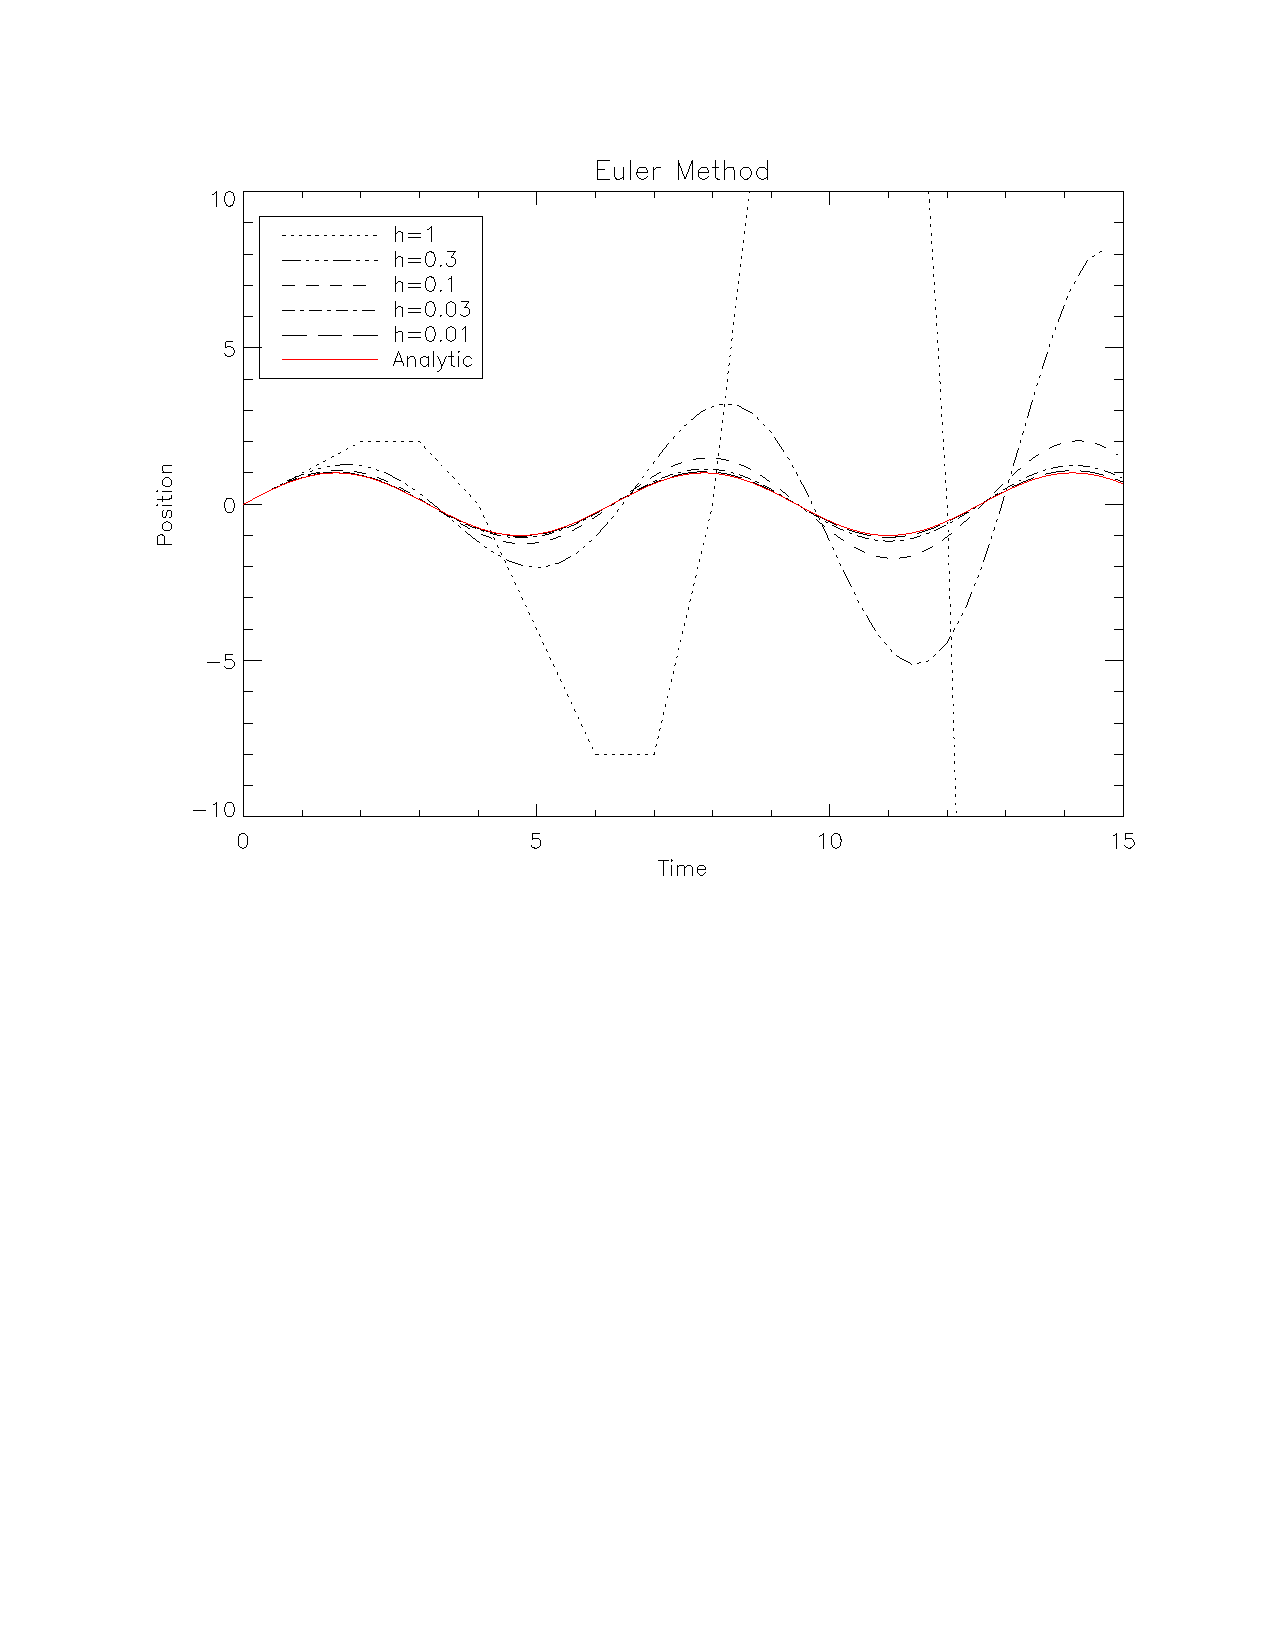
\includegraphics[scale = 0.75]{Euler.pdf}
\caption{}
\end{figure}
\begin{figure}
\centering
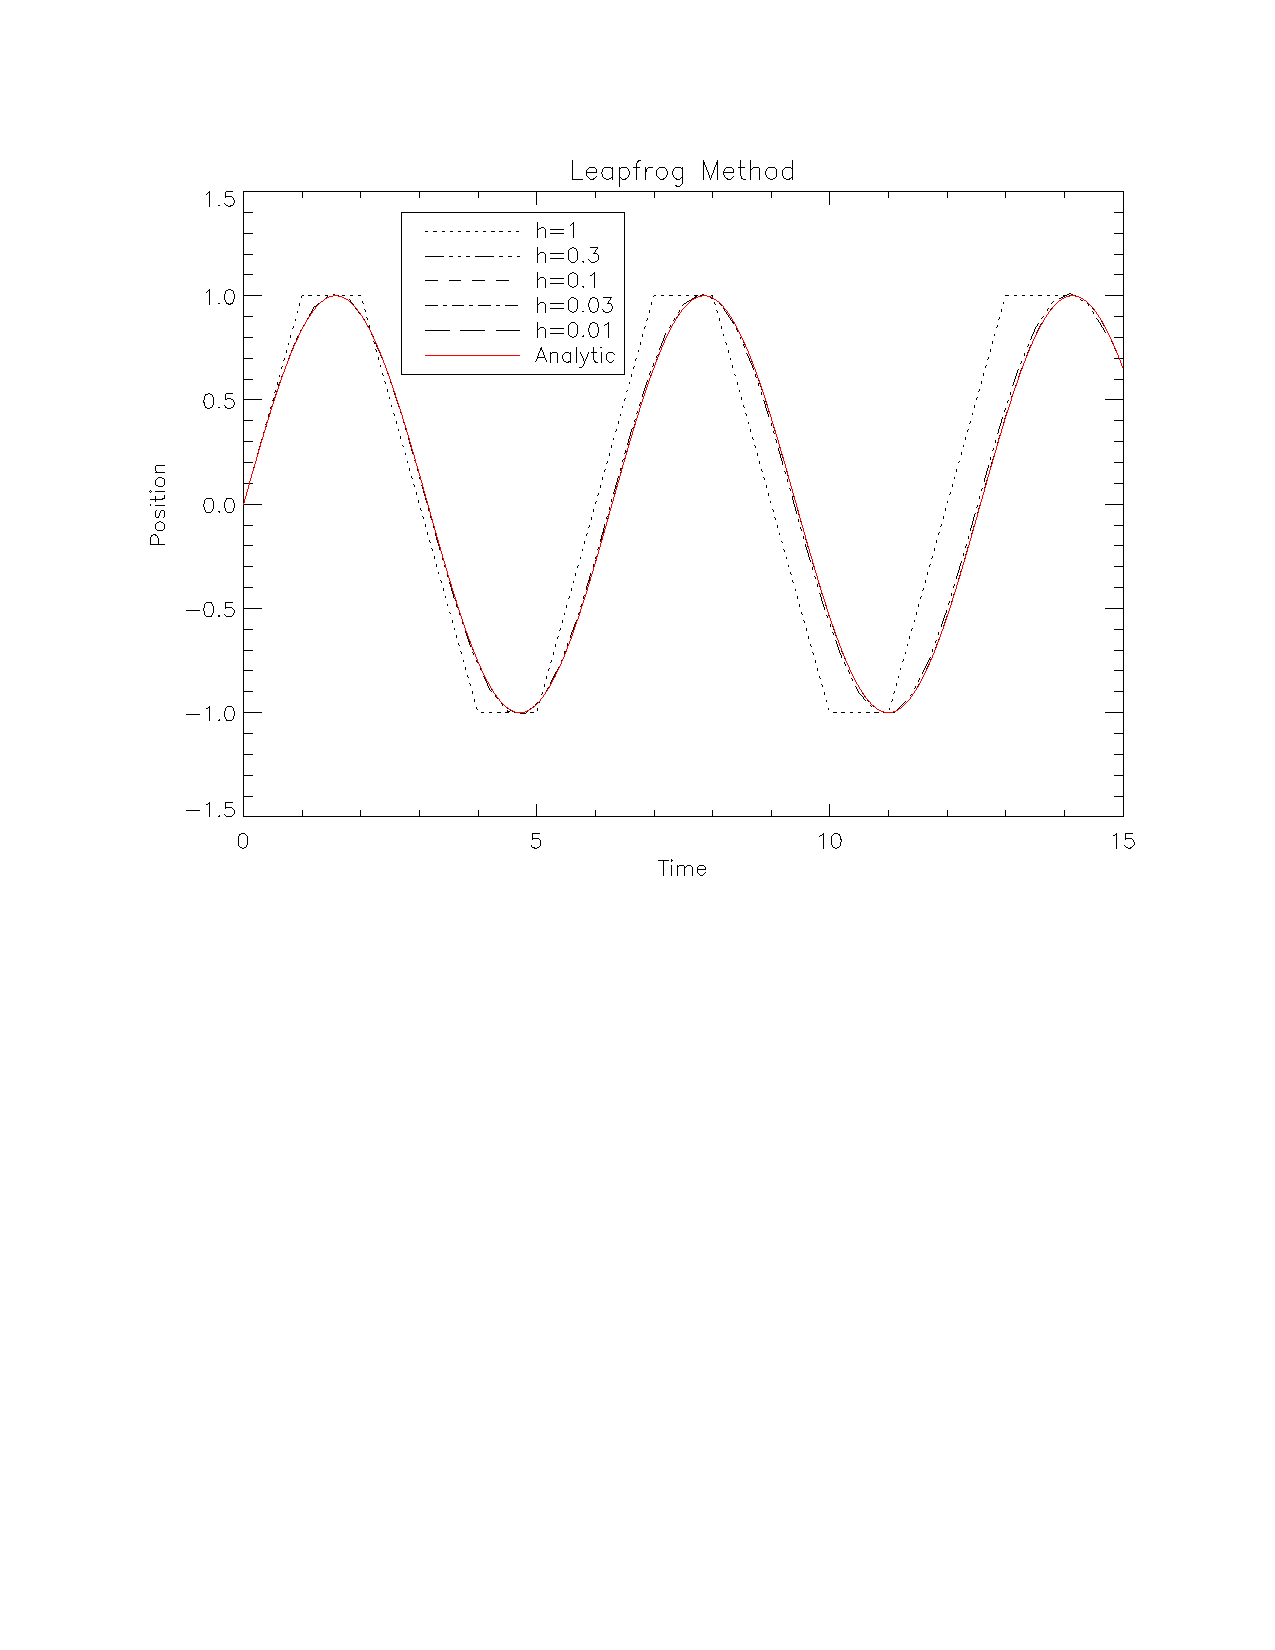
\includegraphics[scale = 0.75]{LF.pdf}
\caption{}
\end{figure}
\begin{figure}
\centering
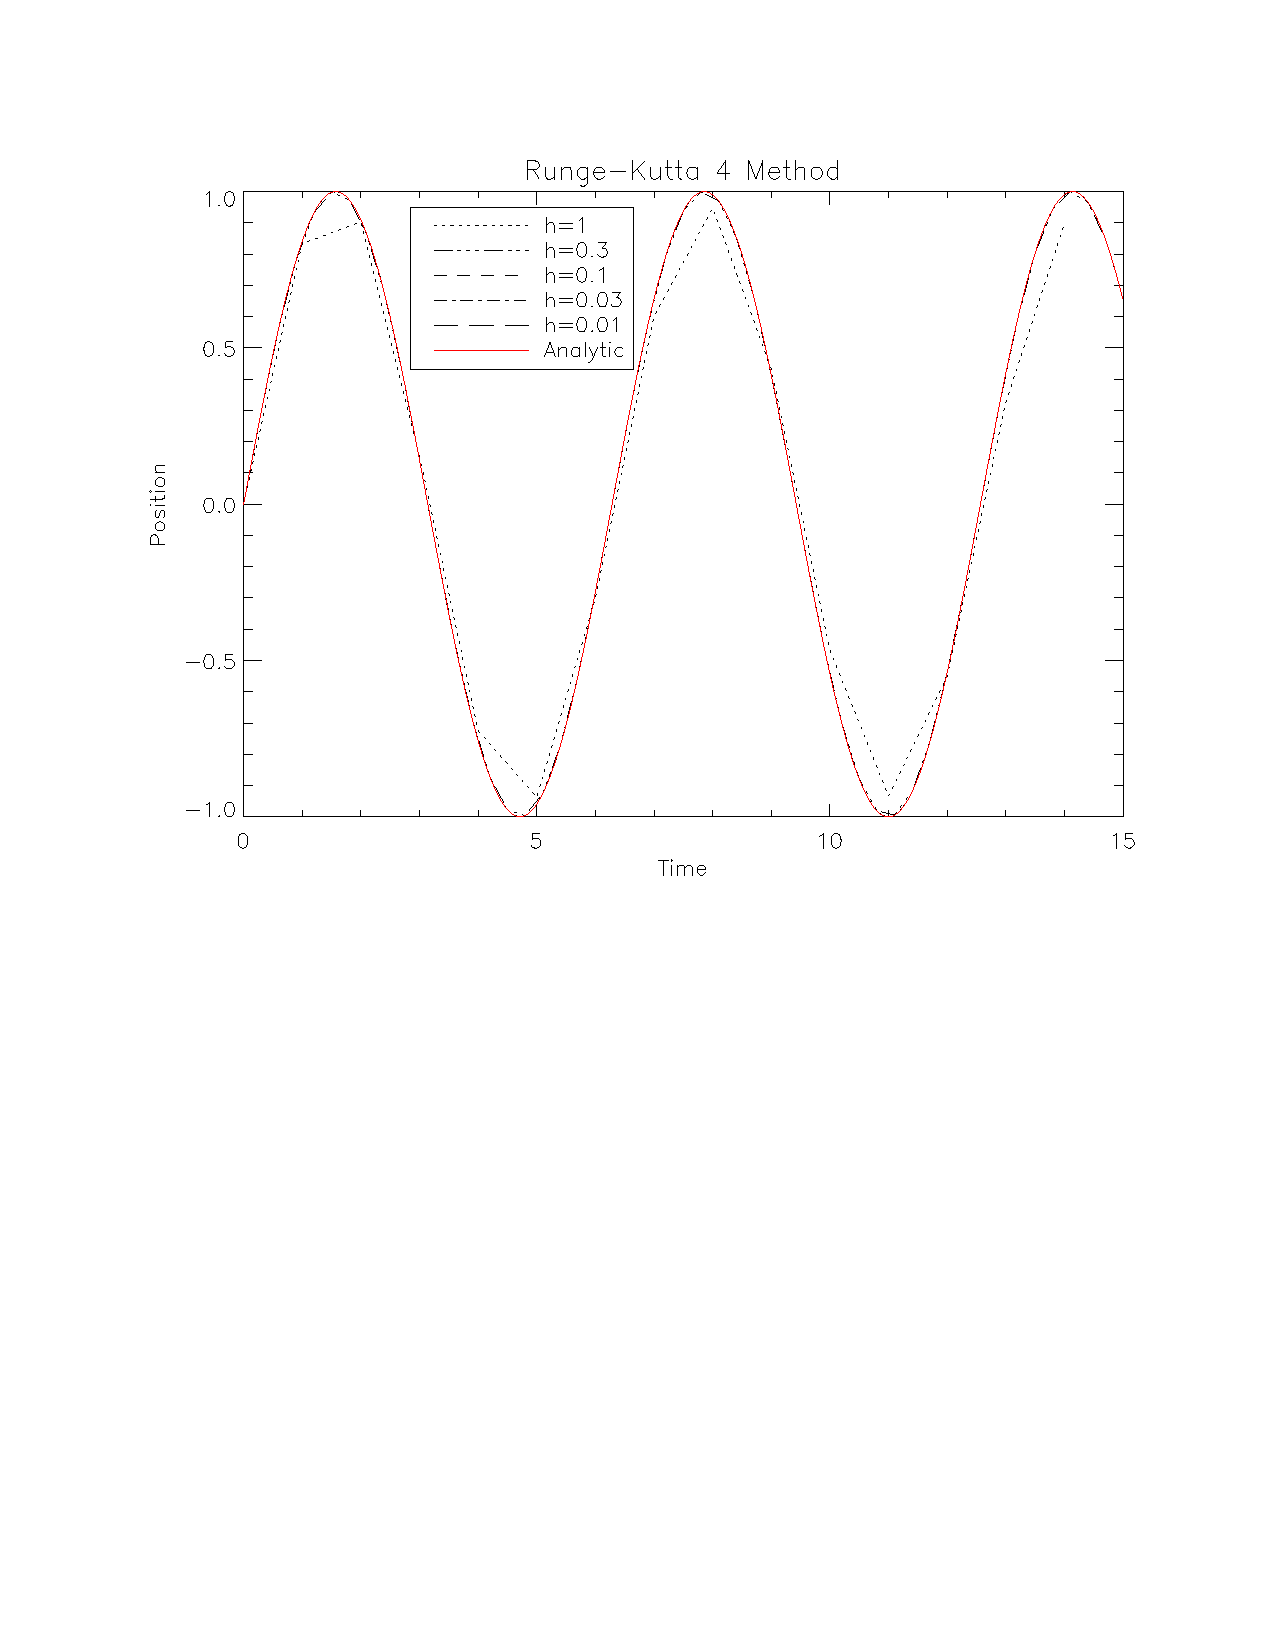
\includegraphics[scale = 0.7]{RK4.pdf}
\caption{}
\end{figure}
\begin{figure}
\centering
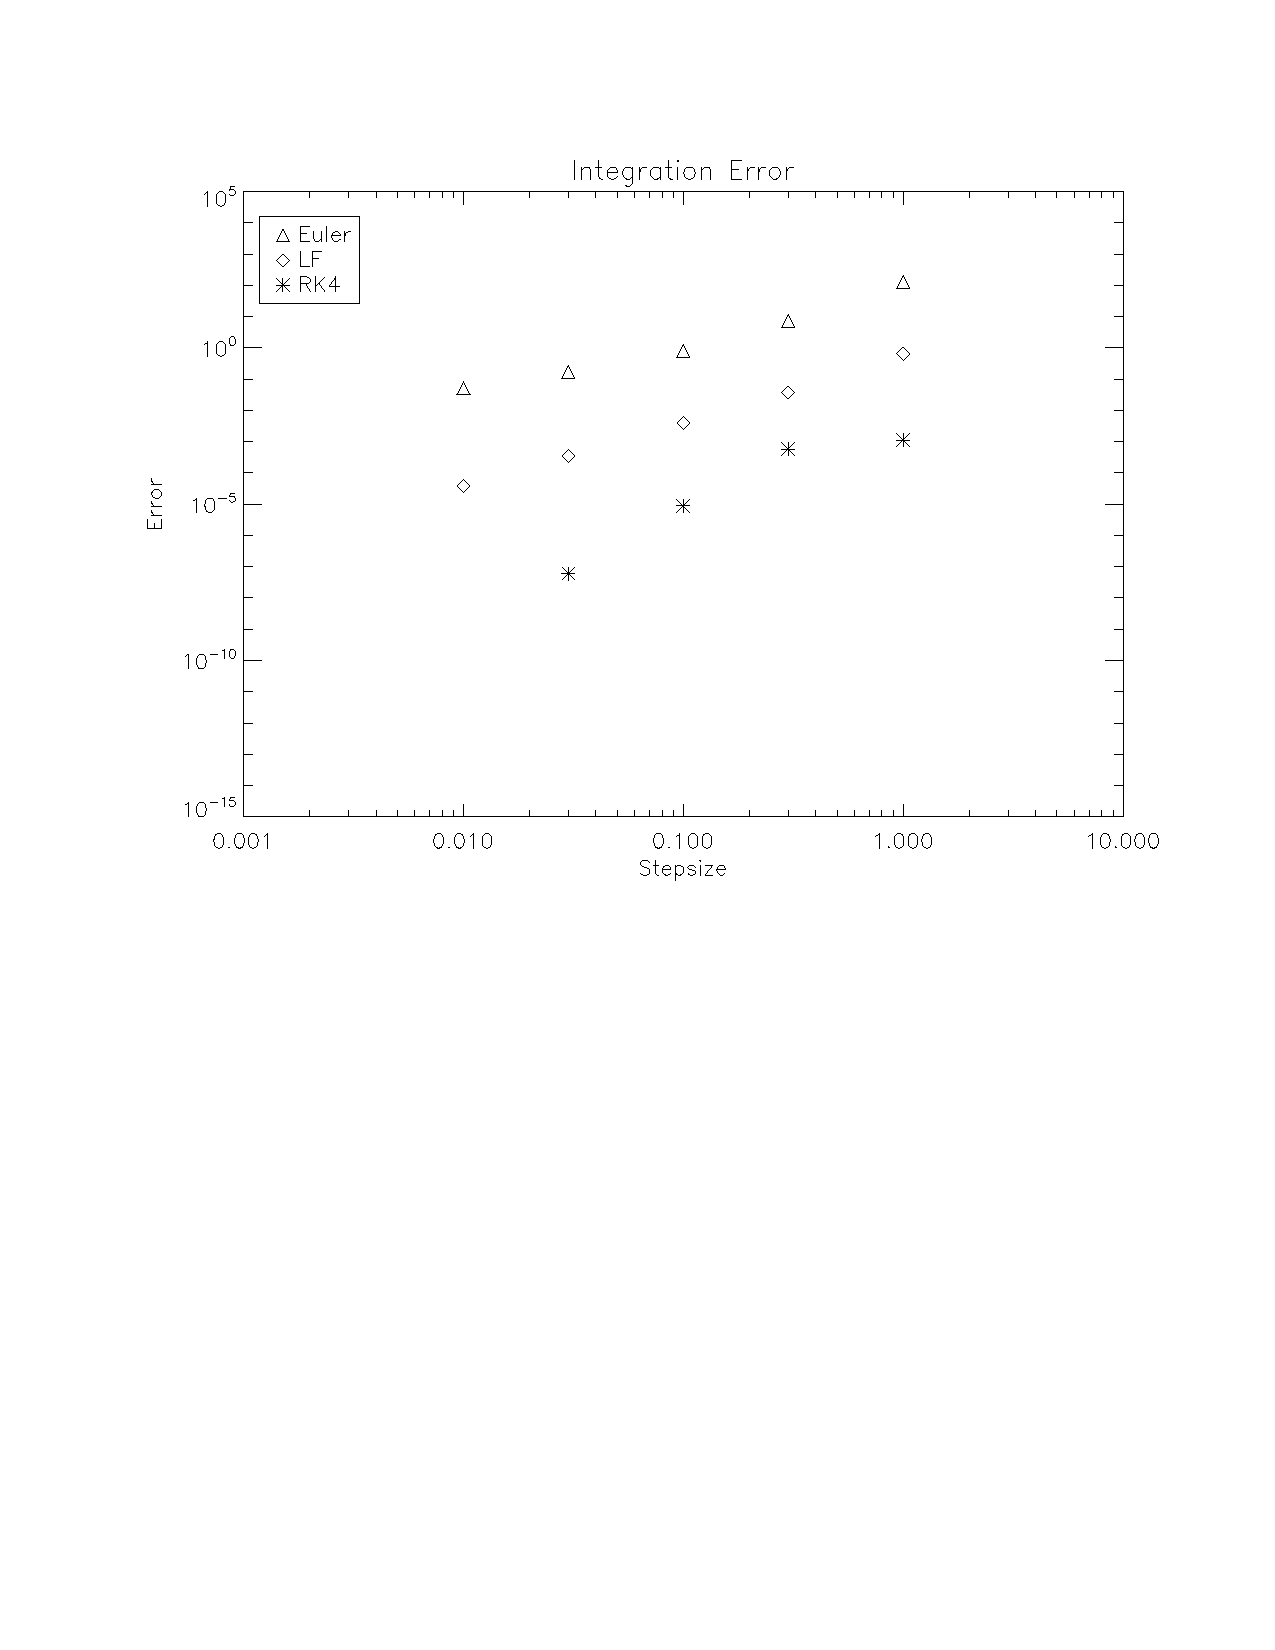
\includegraphics[scale = 0.7]{Error.pdf}
\caption{}
\end{figure}
\begin{figure}
\begin{center}$
\begin{array}{cc}
\hspace*{-1in}
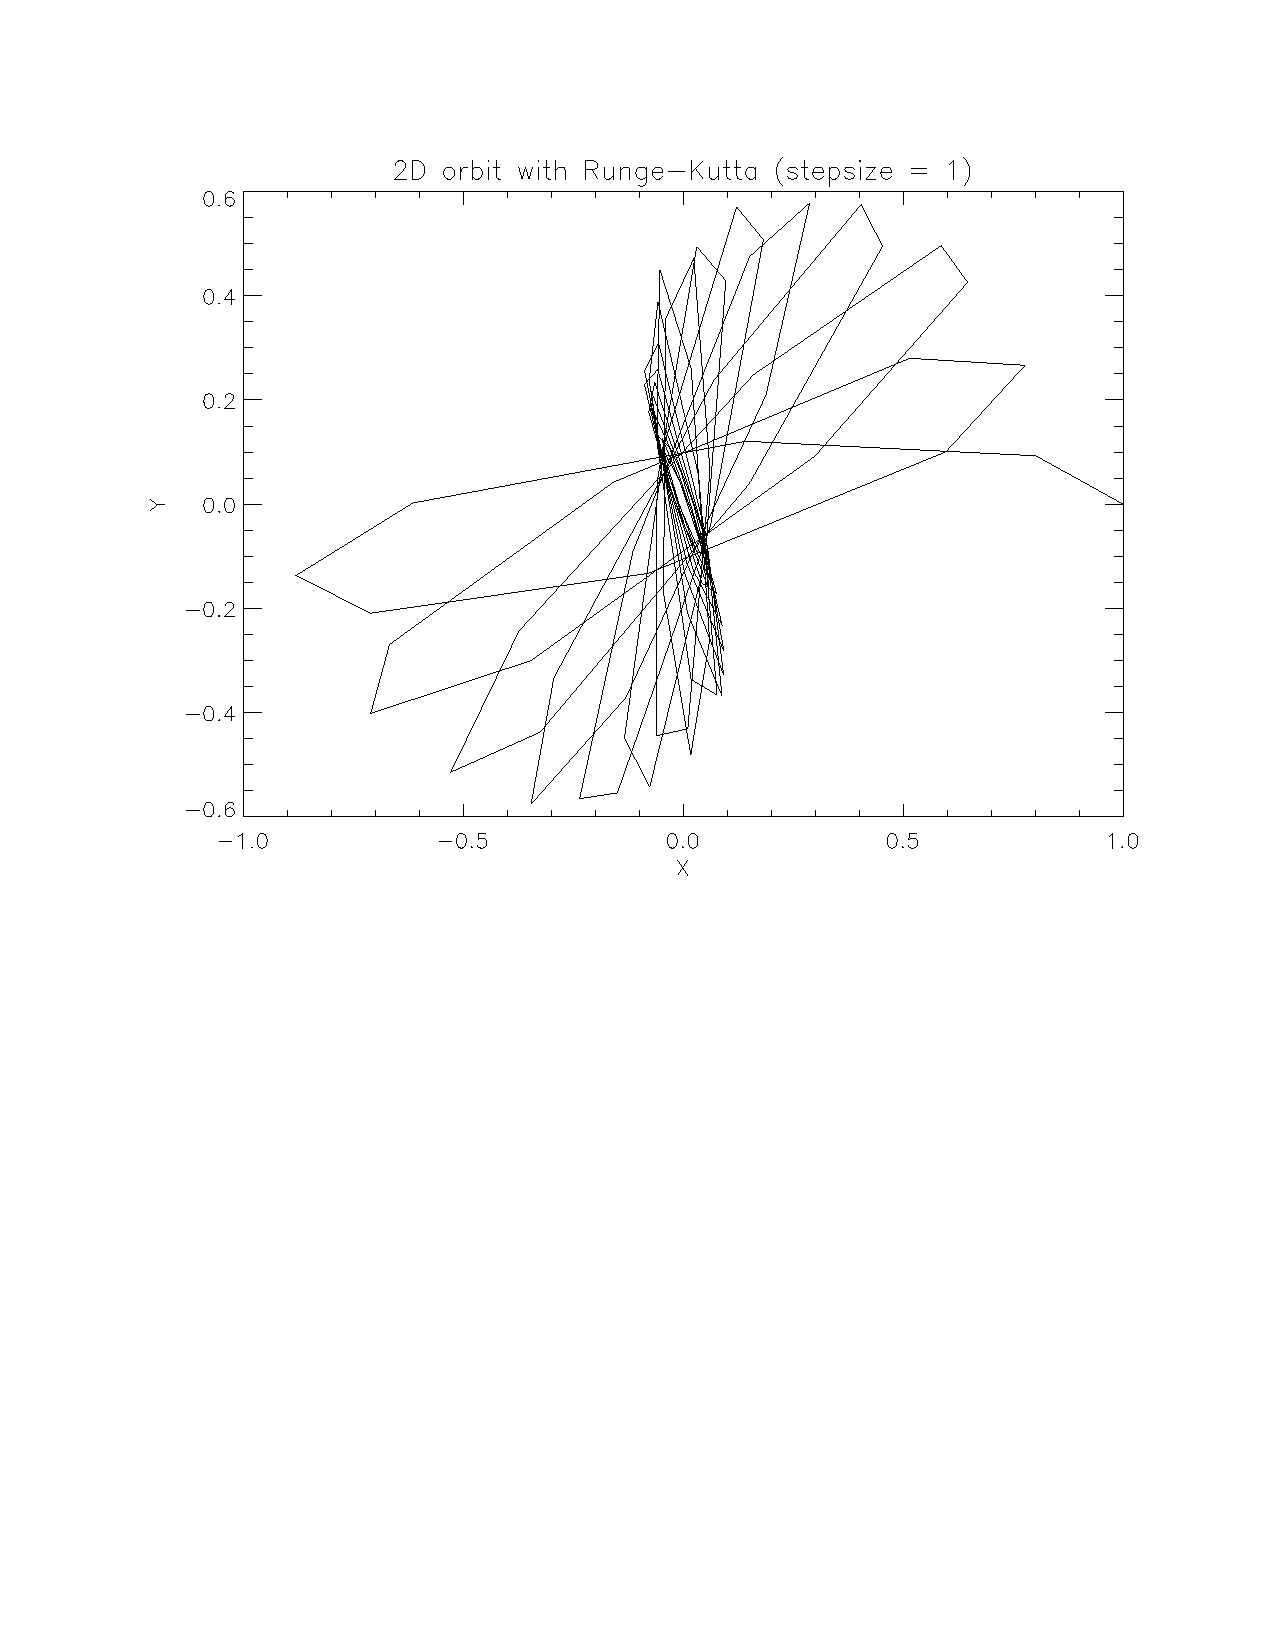
\includegraphics[height = 4in, width = 4in]{Orbit_RK_10.pdf} &
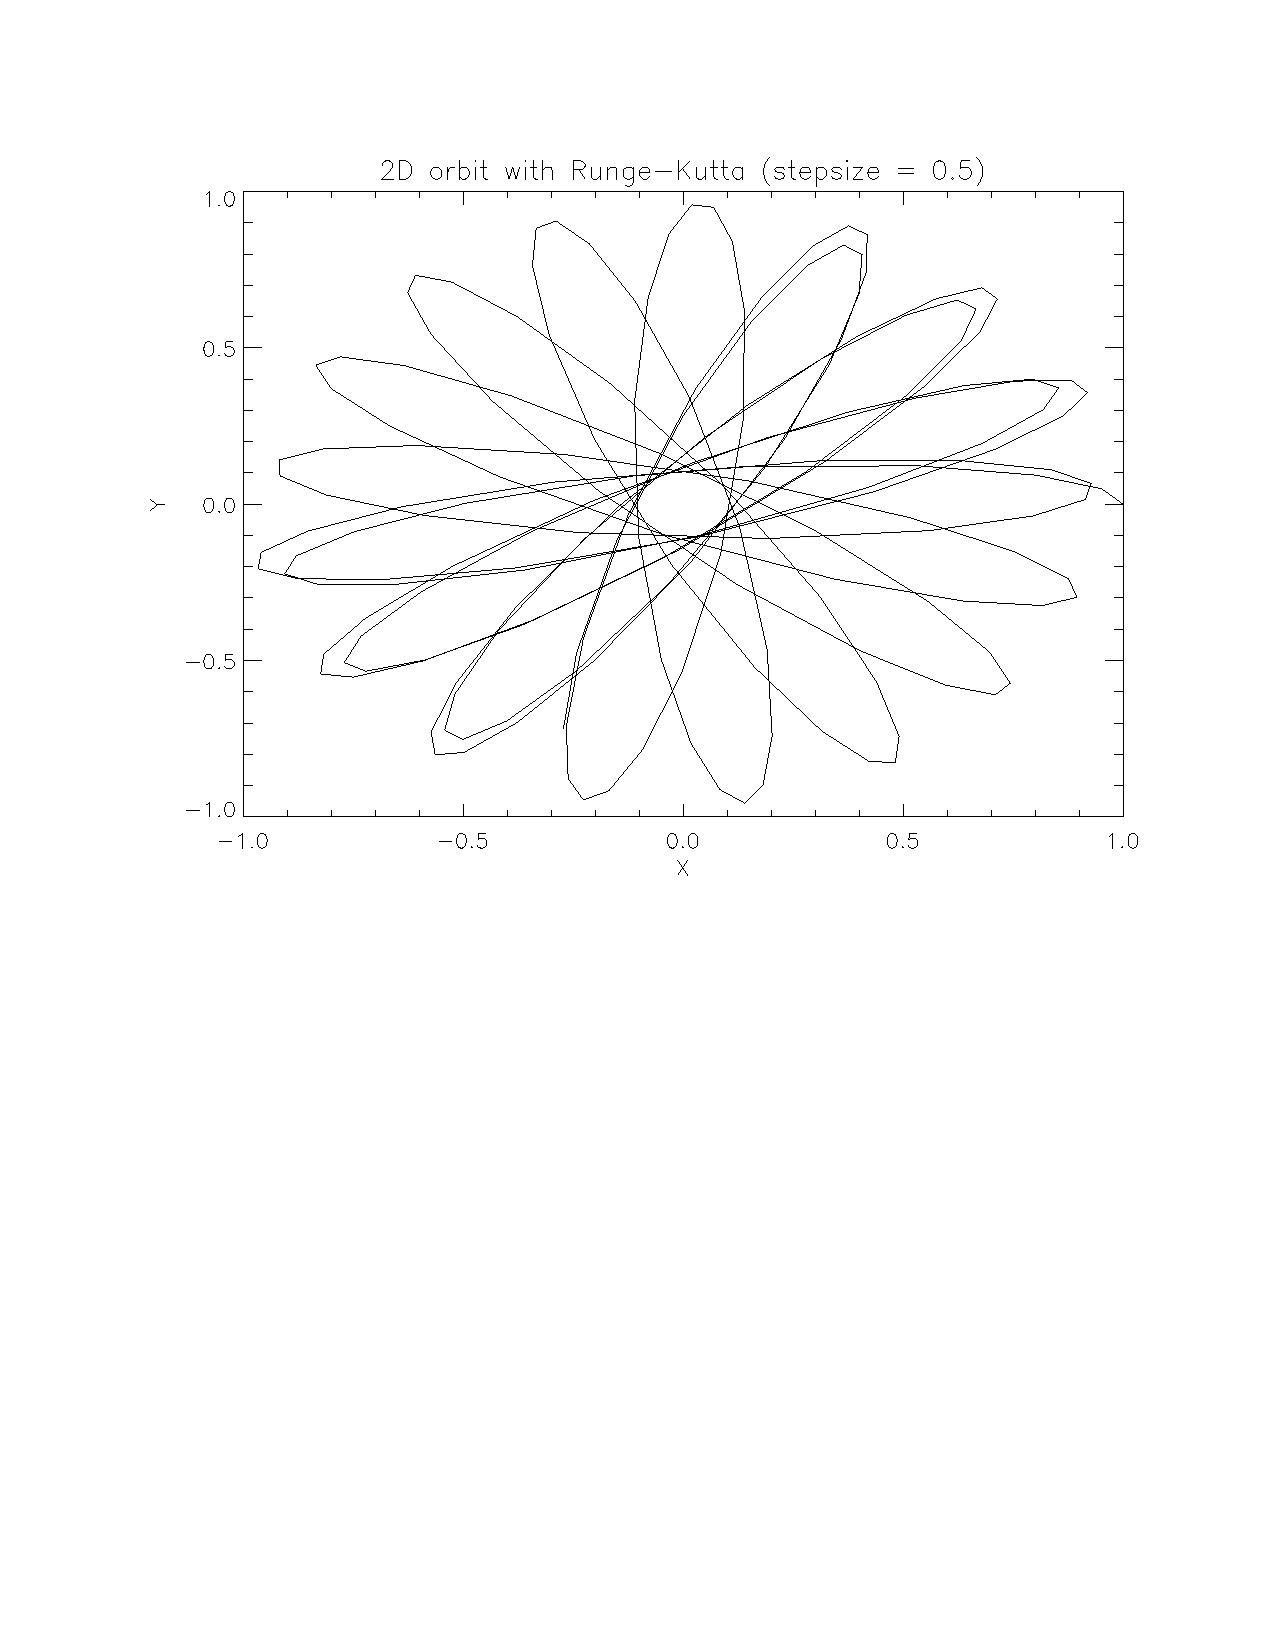
\includegraphics[height = 4in, width = 4in ]{Orbit_RK_5.pdf} \\ 
\hspace*{-1in}
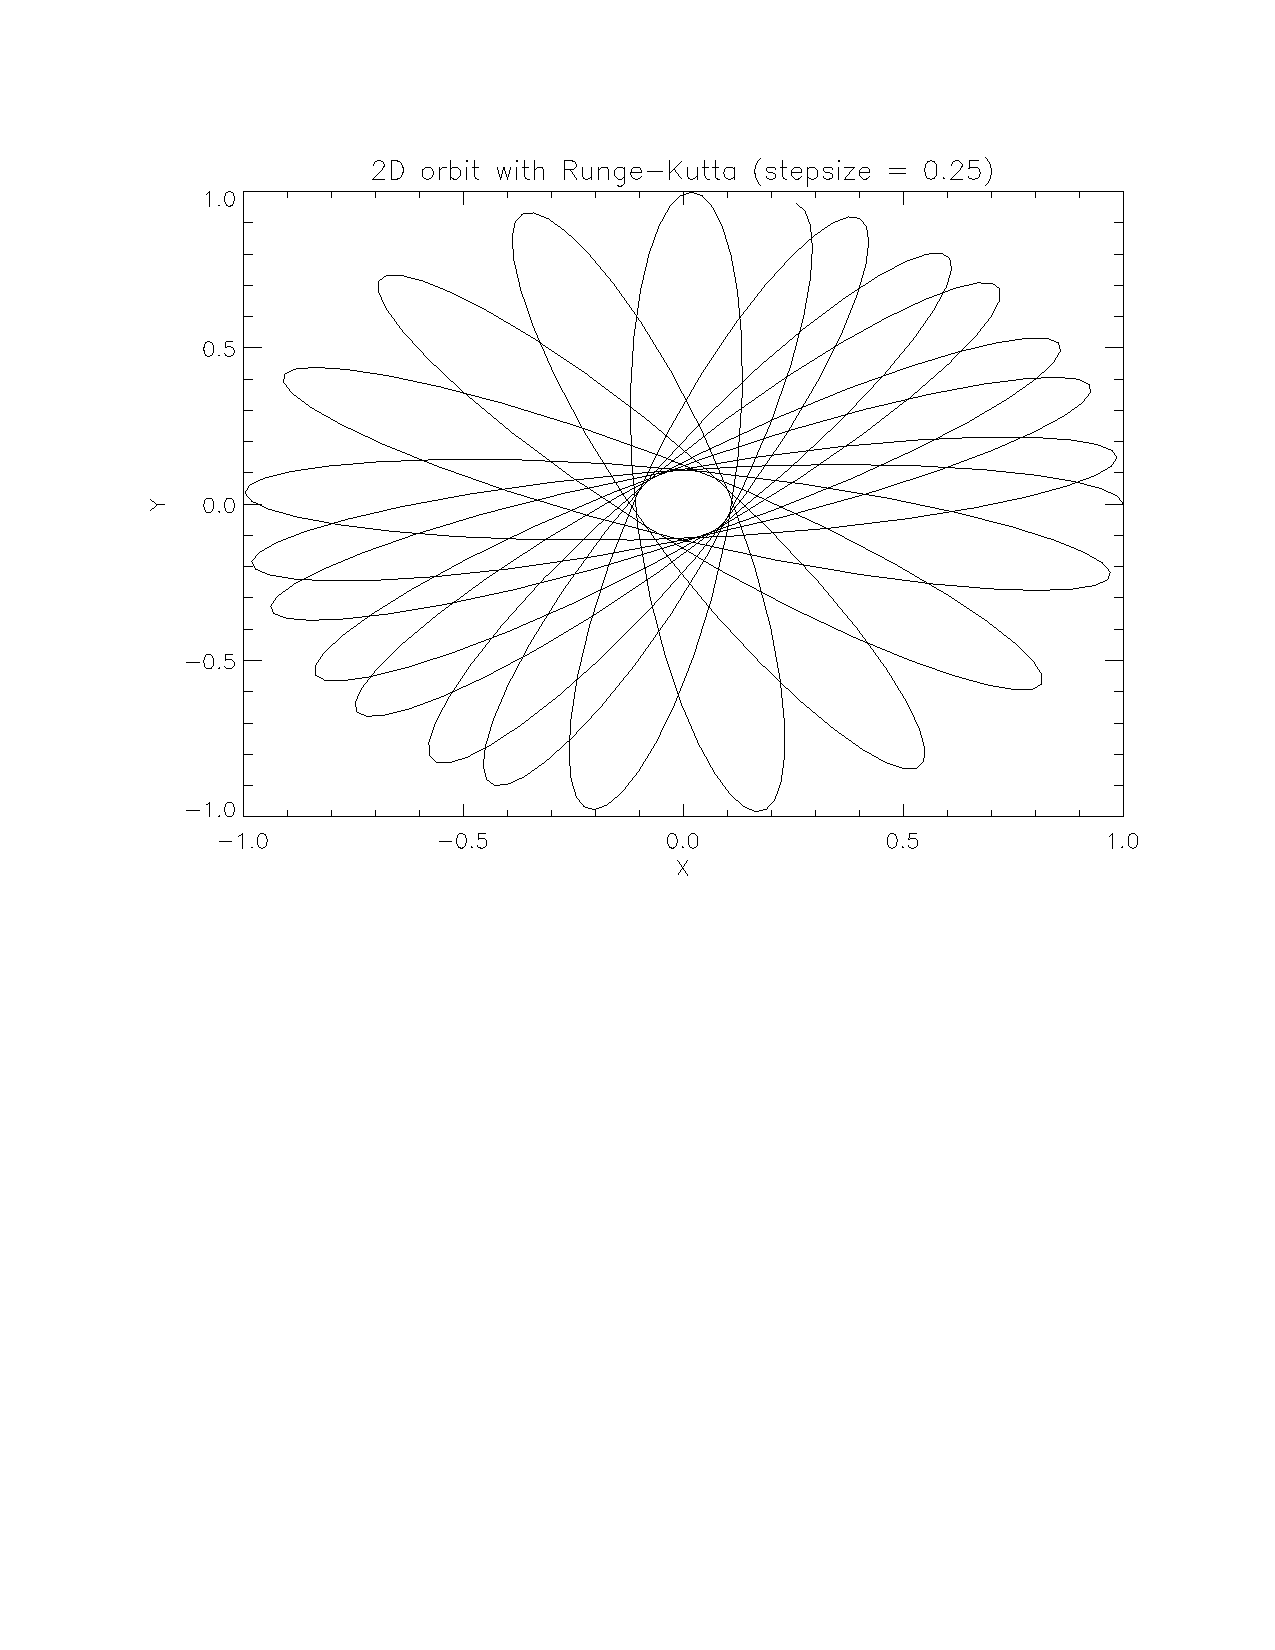
\includegraphics[height = 4in, width = 4in]{Orbit_RK_25.pdf} &
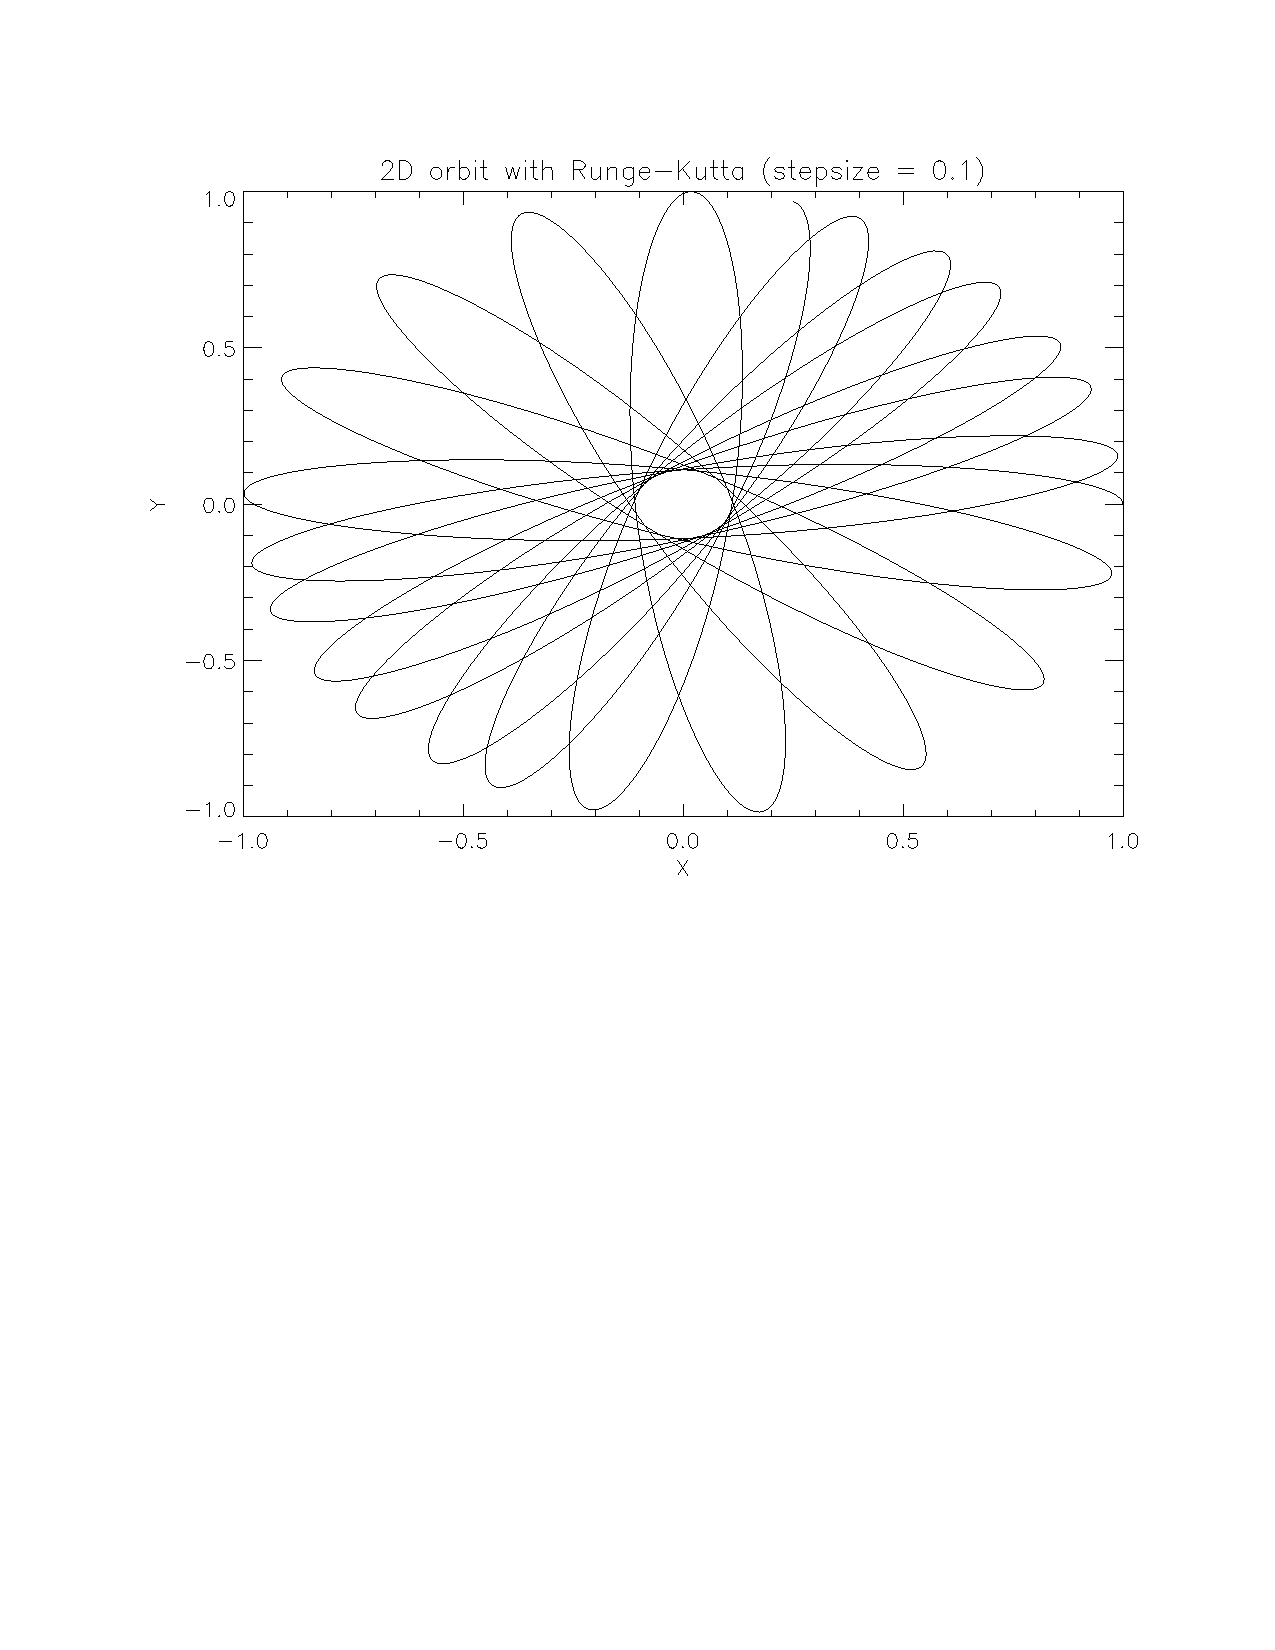
\includegraphics[height = 4in, width = 4in]{Orbit_RK_1.pdf}
\end{array}$
\end{center}
\caption{}
\end{figure}
\begin{figure}
\begin{center}$
\begin{array}{cc}
\hspace*{-1in}
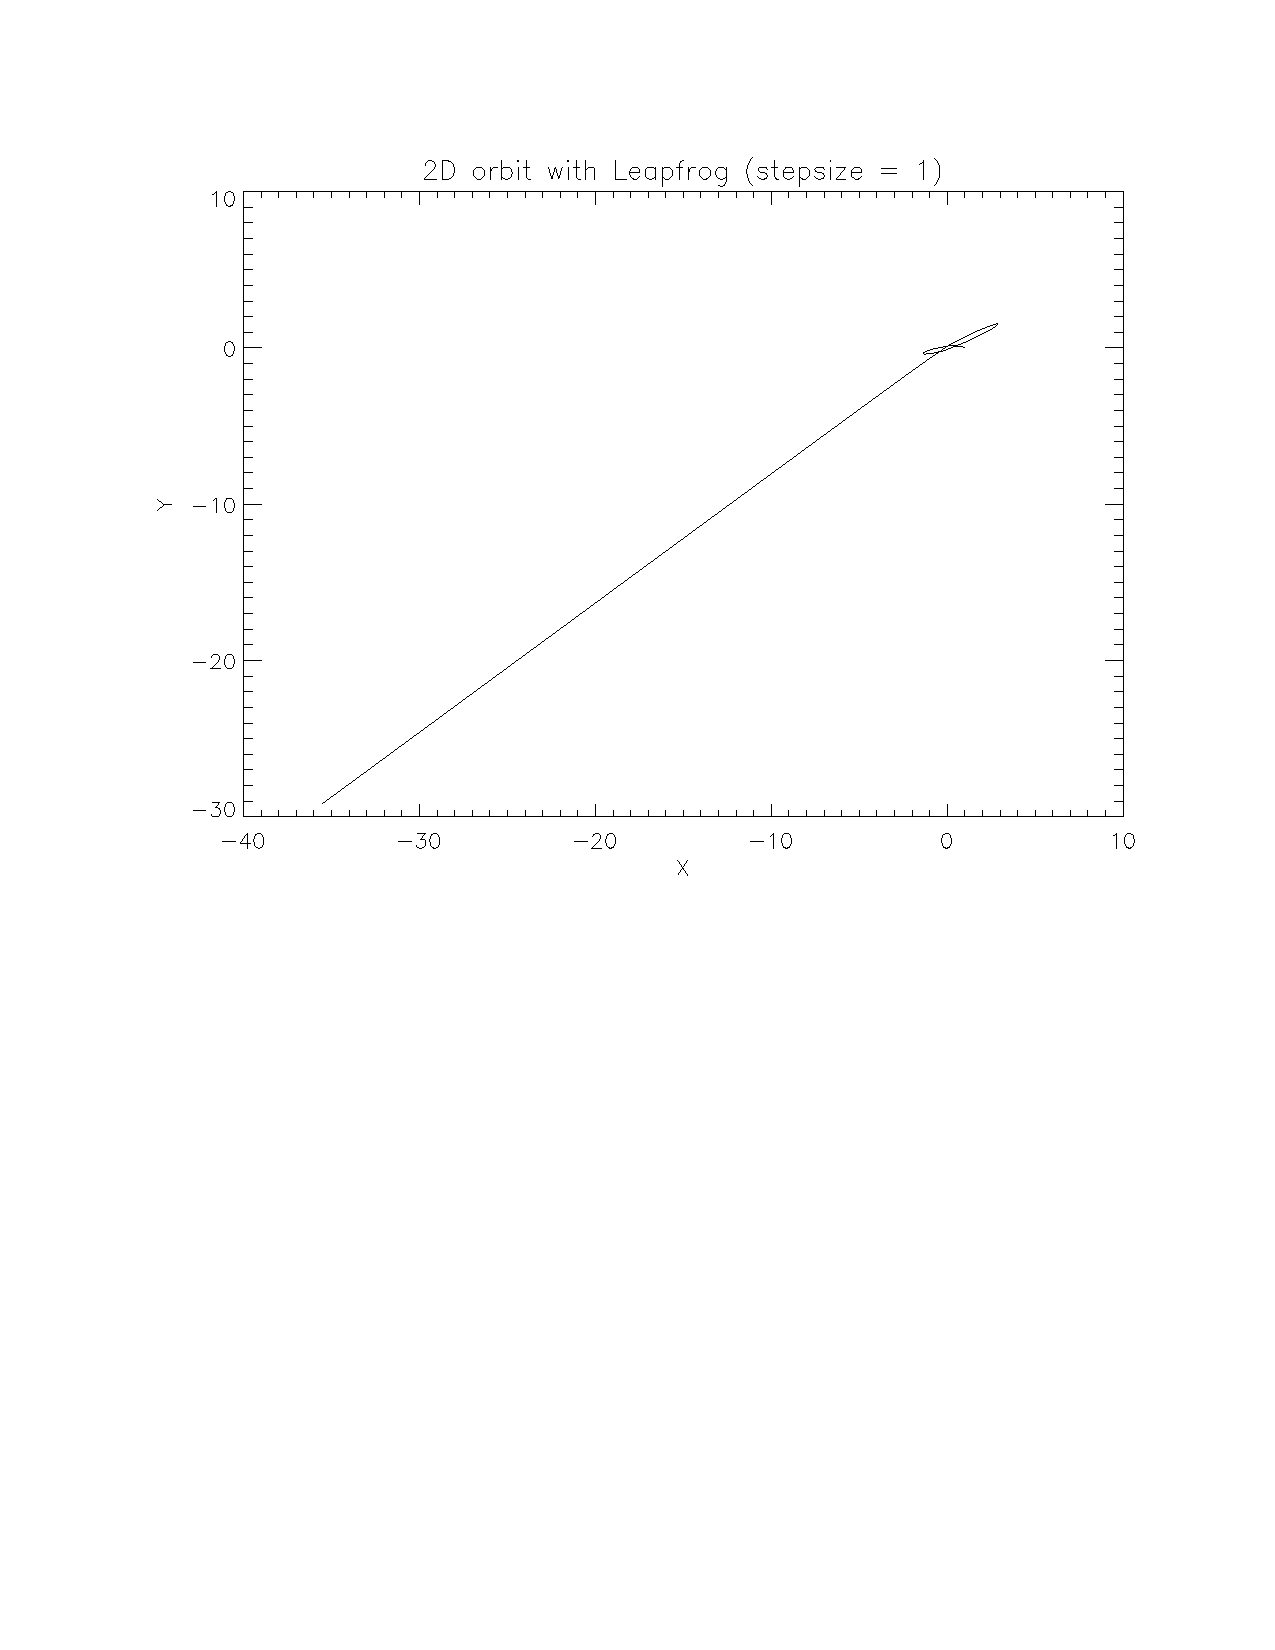
\includegraphics[height = 4in, width = 4in]{Orbit_LF_10.pdf} &
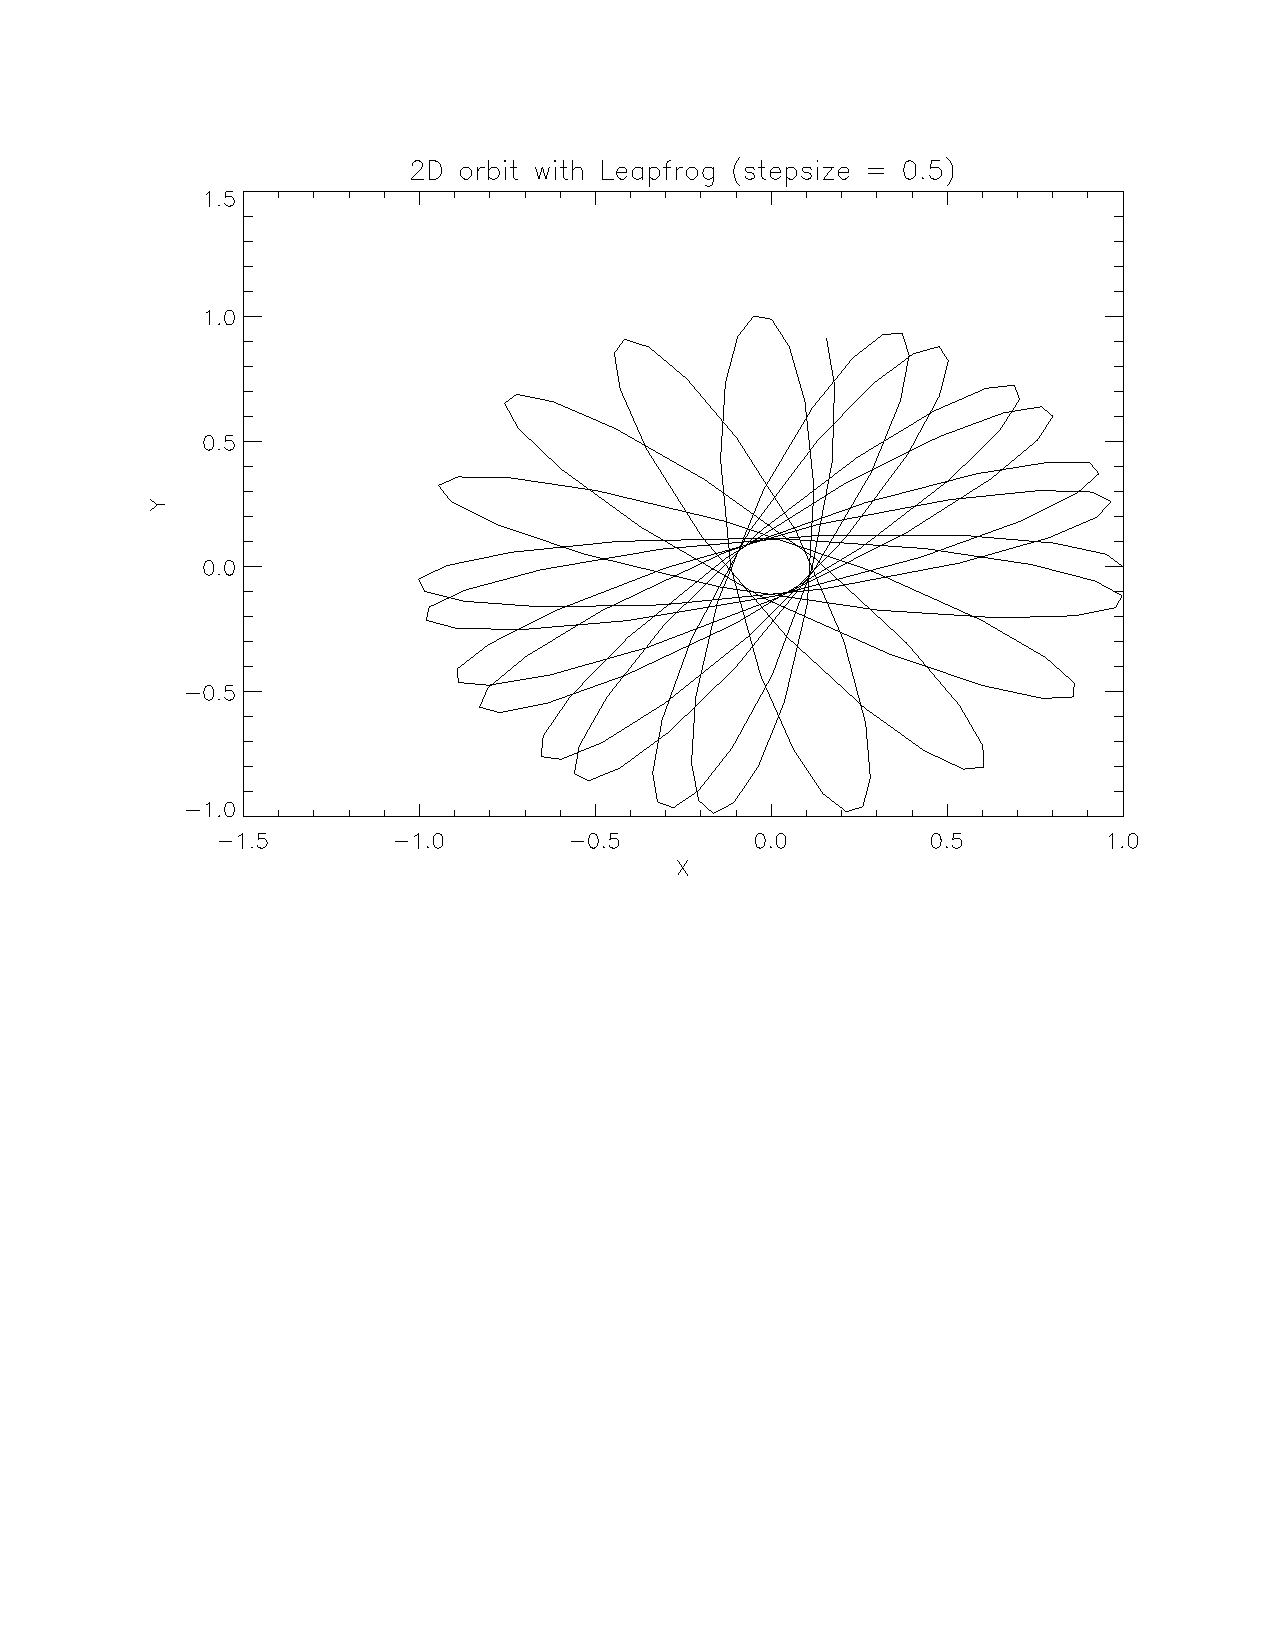
\includegraphics[height = 4in, width = 4in ]{Orbit_LF_5.pdf} \\ 
\hspace*{-1in}
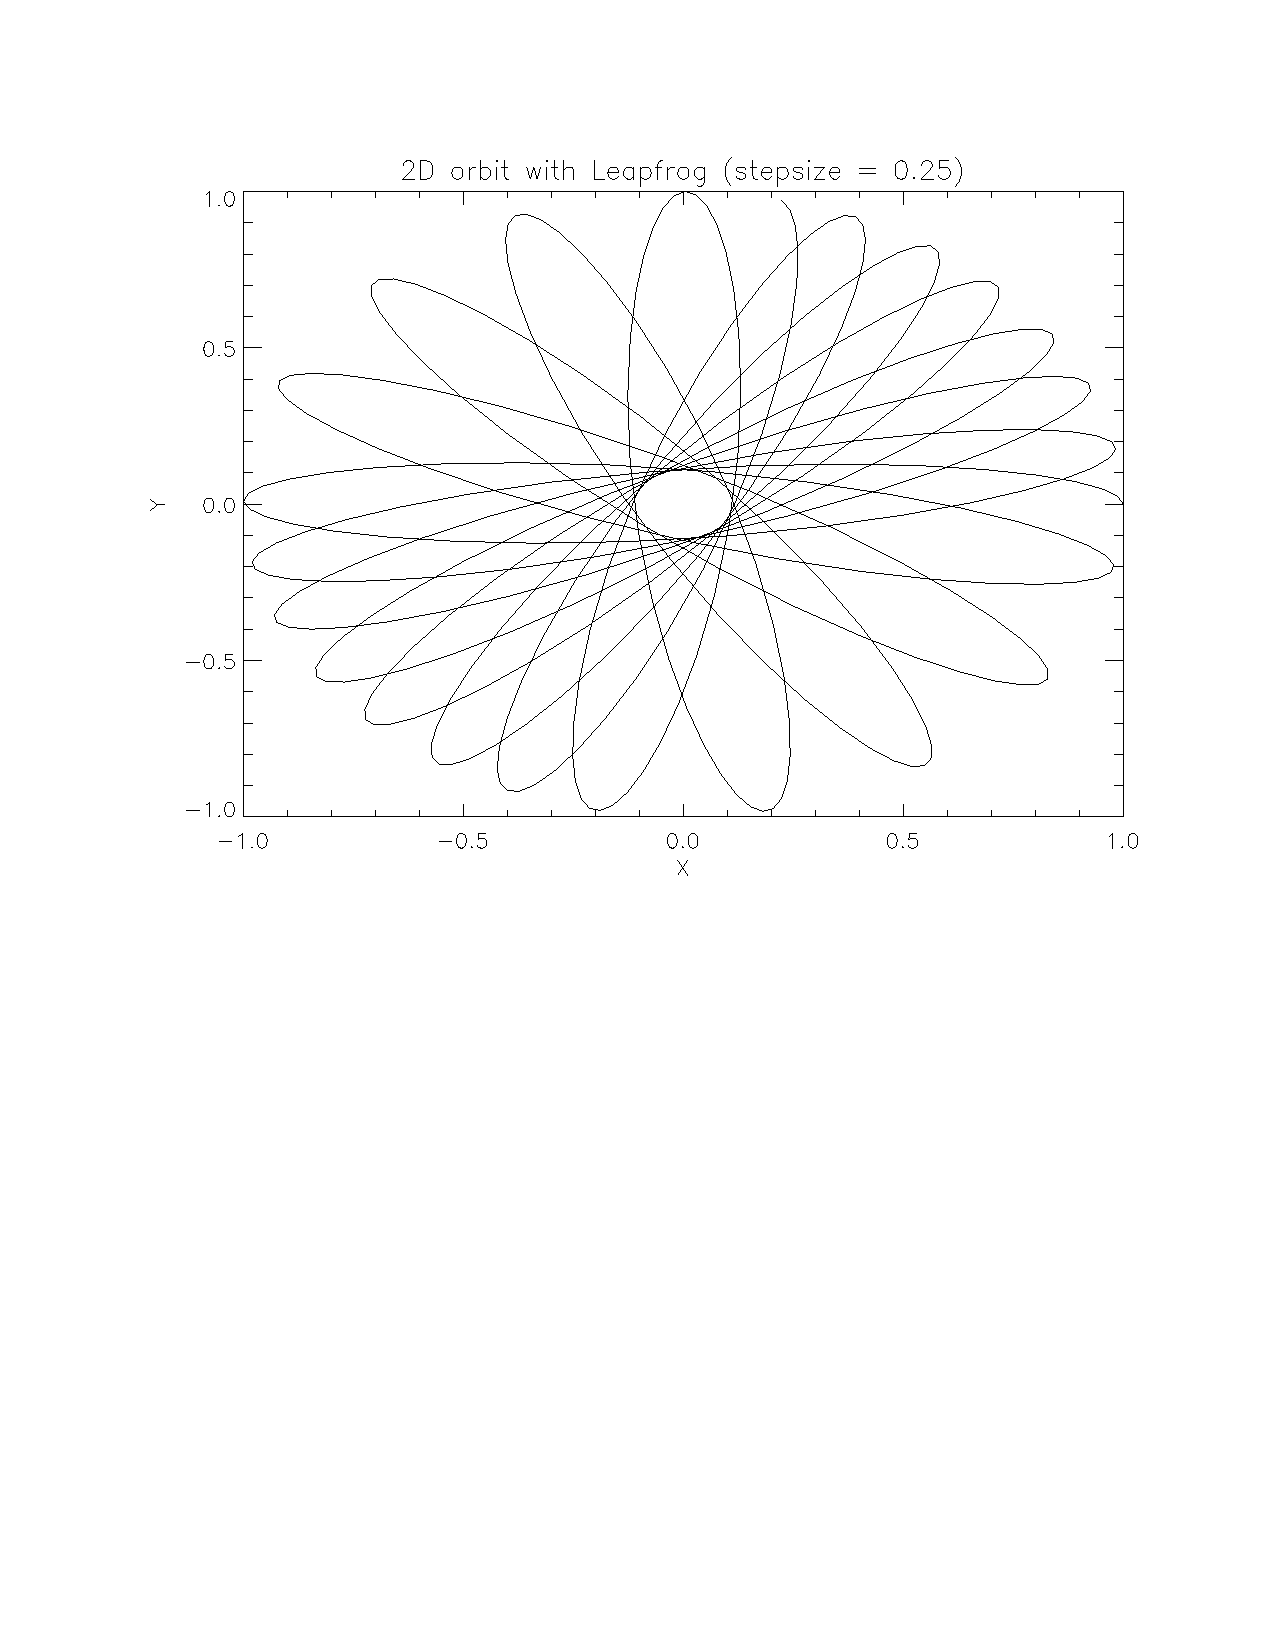
\includegraphics[height = 4in, width = 4in]{Orbit_LF_25.pdf} &
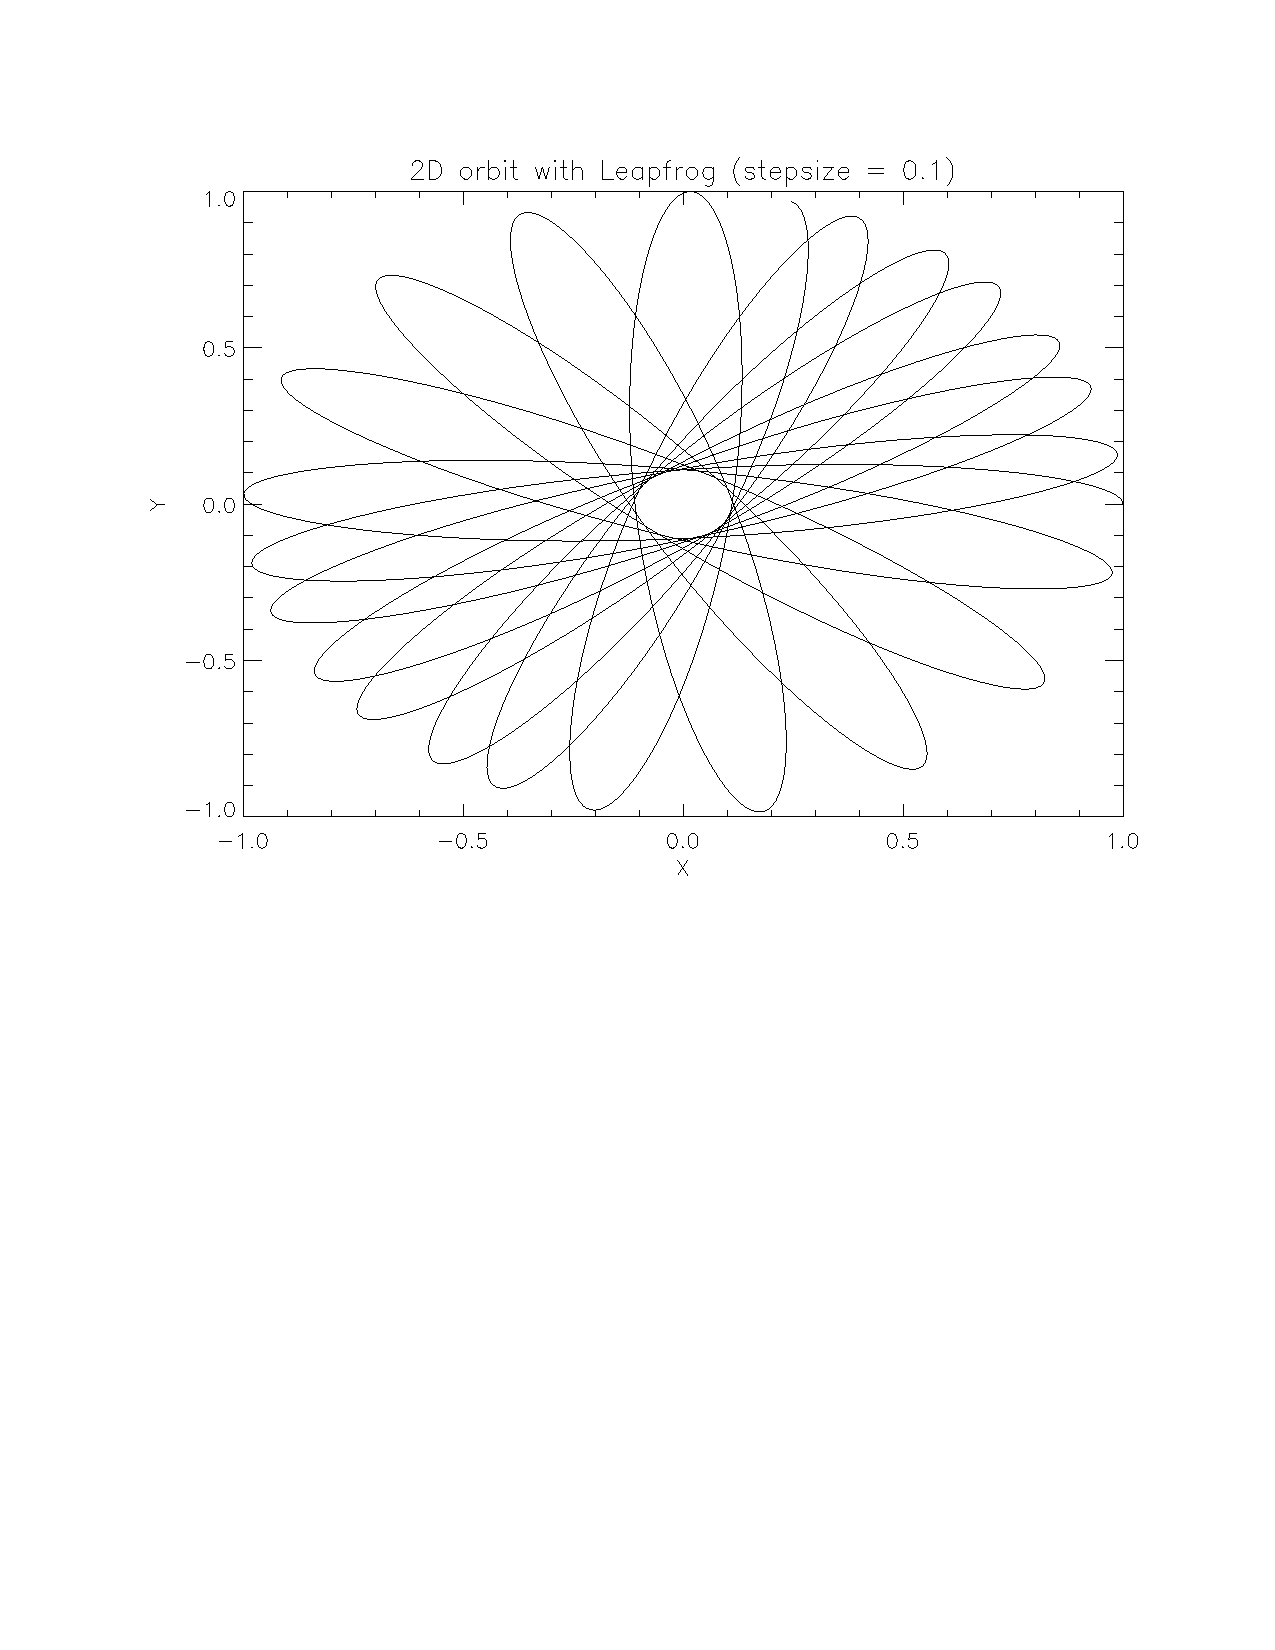
\includegraphics[height = 4in, width = 4in]{Orbit_LF_1.pdf}
\end{array}$
\end{center}
\caption{}
\end{figure}
\begin{figure}
\centering
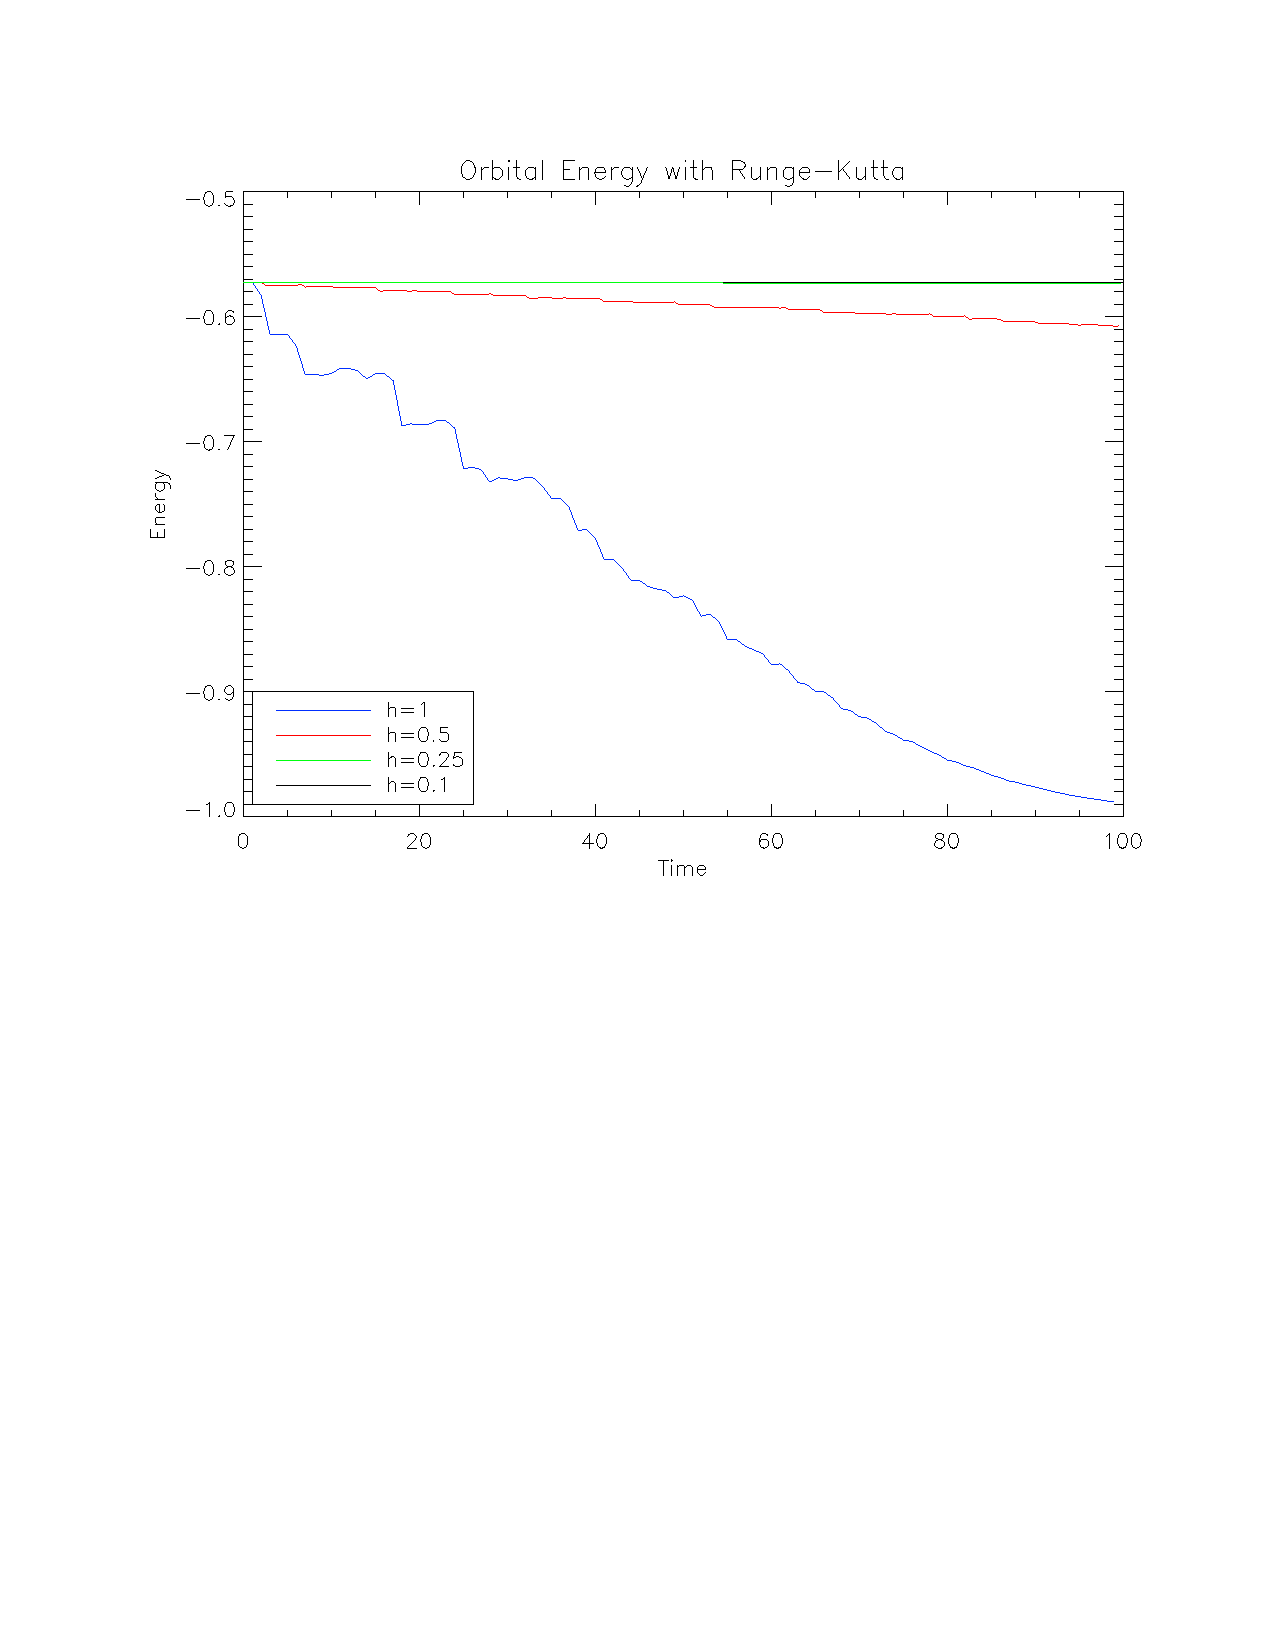
\includegraphics[scale = 0.75]{RKEnergy.pdf}
\caption{}
\end{figure}
\begin{figure}
\centering
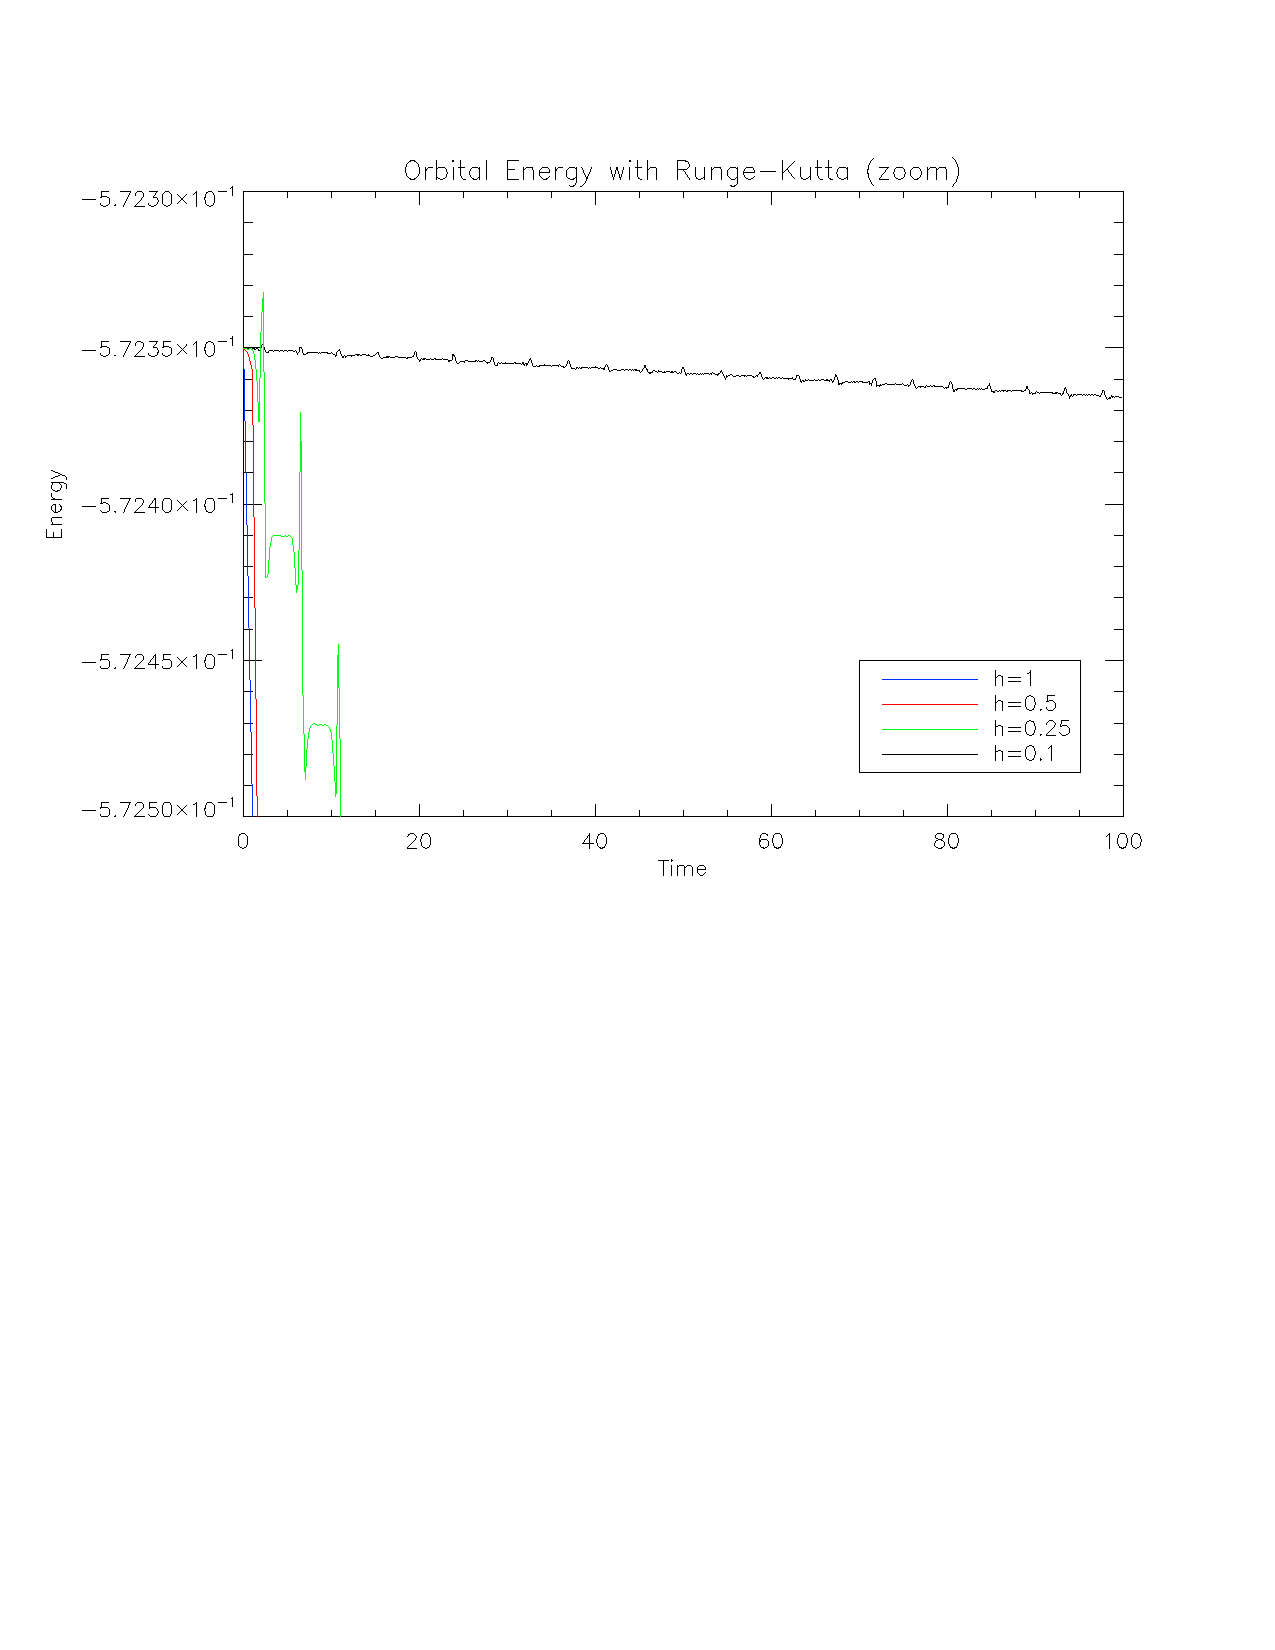
\includegraphics[scale = 0.75]{RKEnzoom.pdf}
\caption{}
\end{figure}
\begin{figure}
\centering
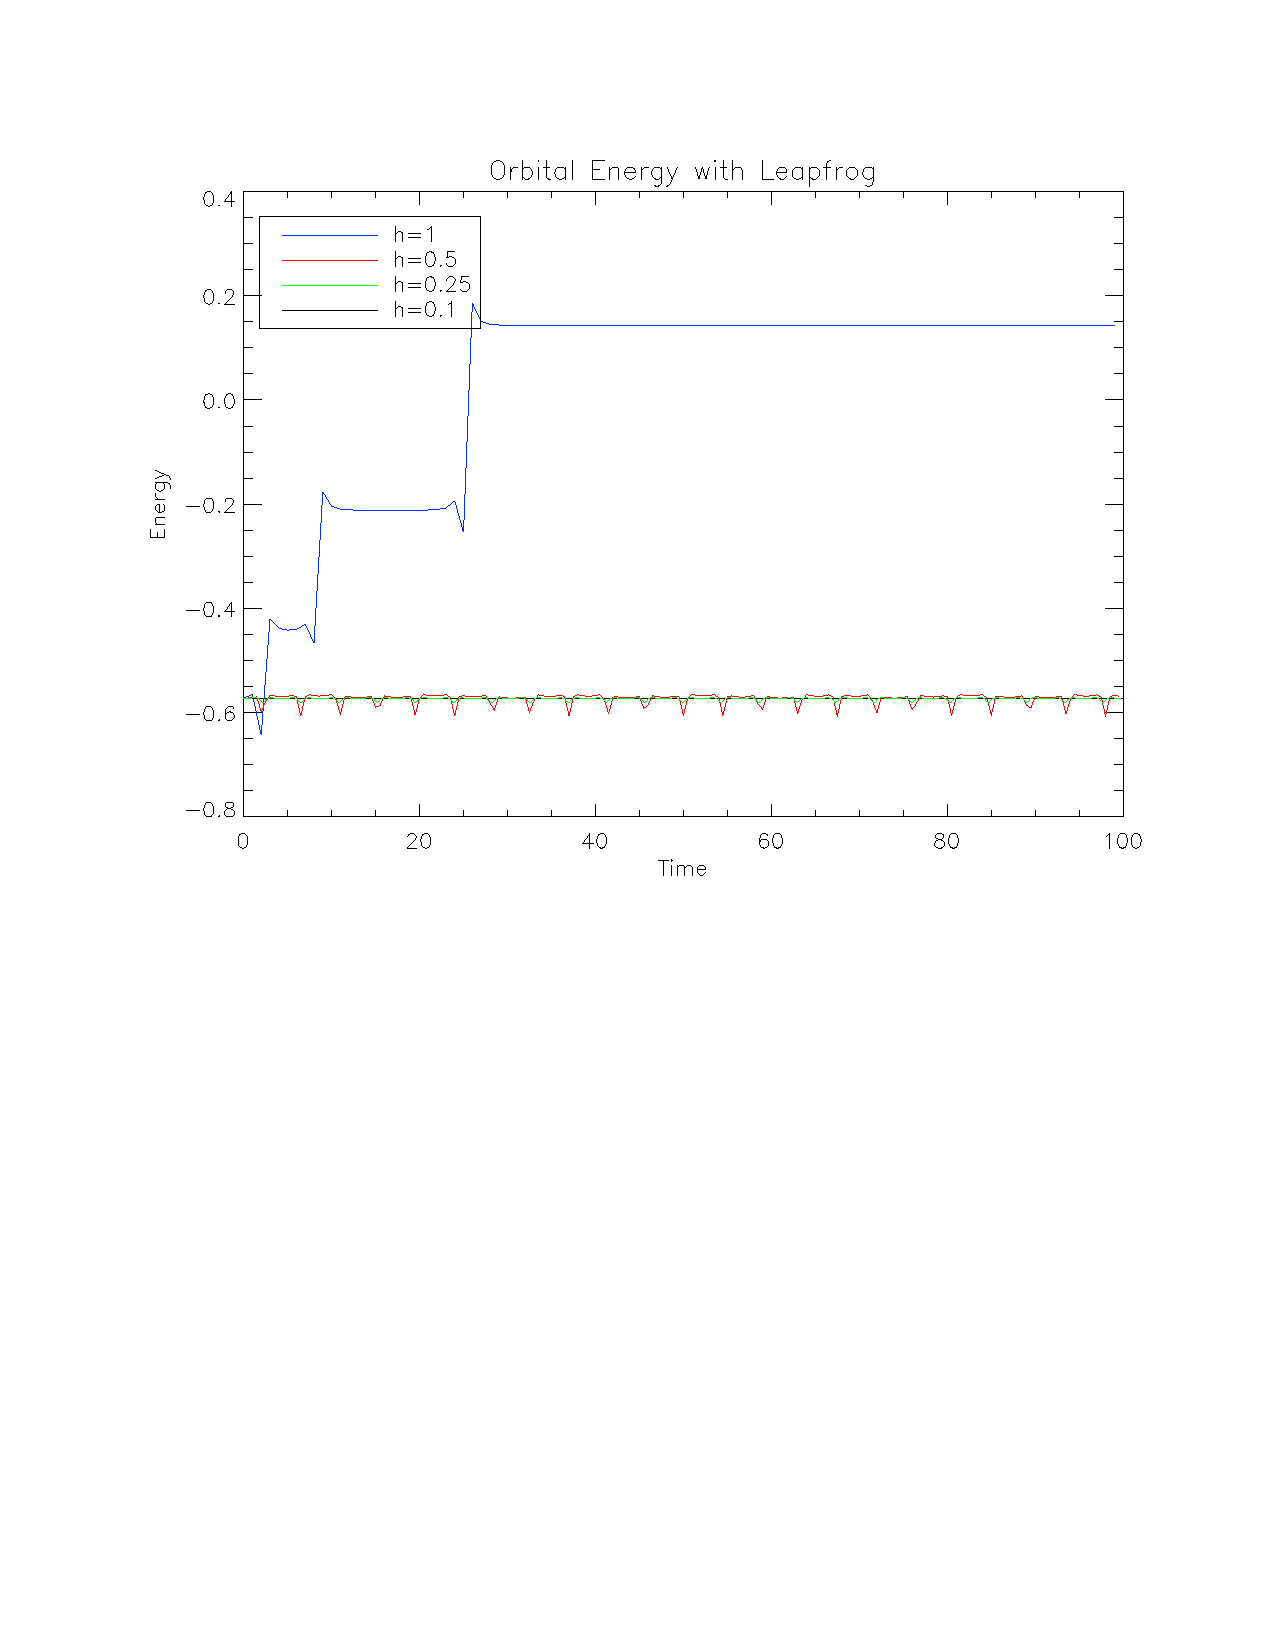
\includegraphics[scale = 0.7]{LFEnergy.pdf}
\caption{}
\end{figure}
\begin{figure}
\centering
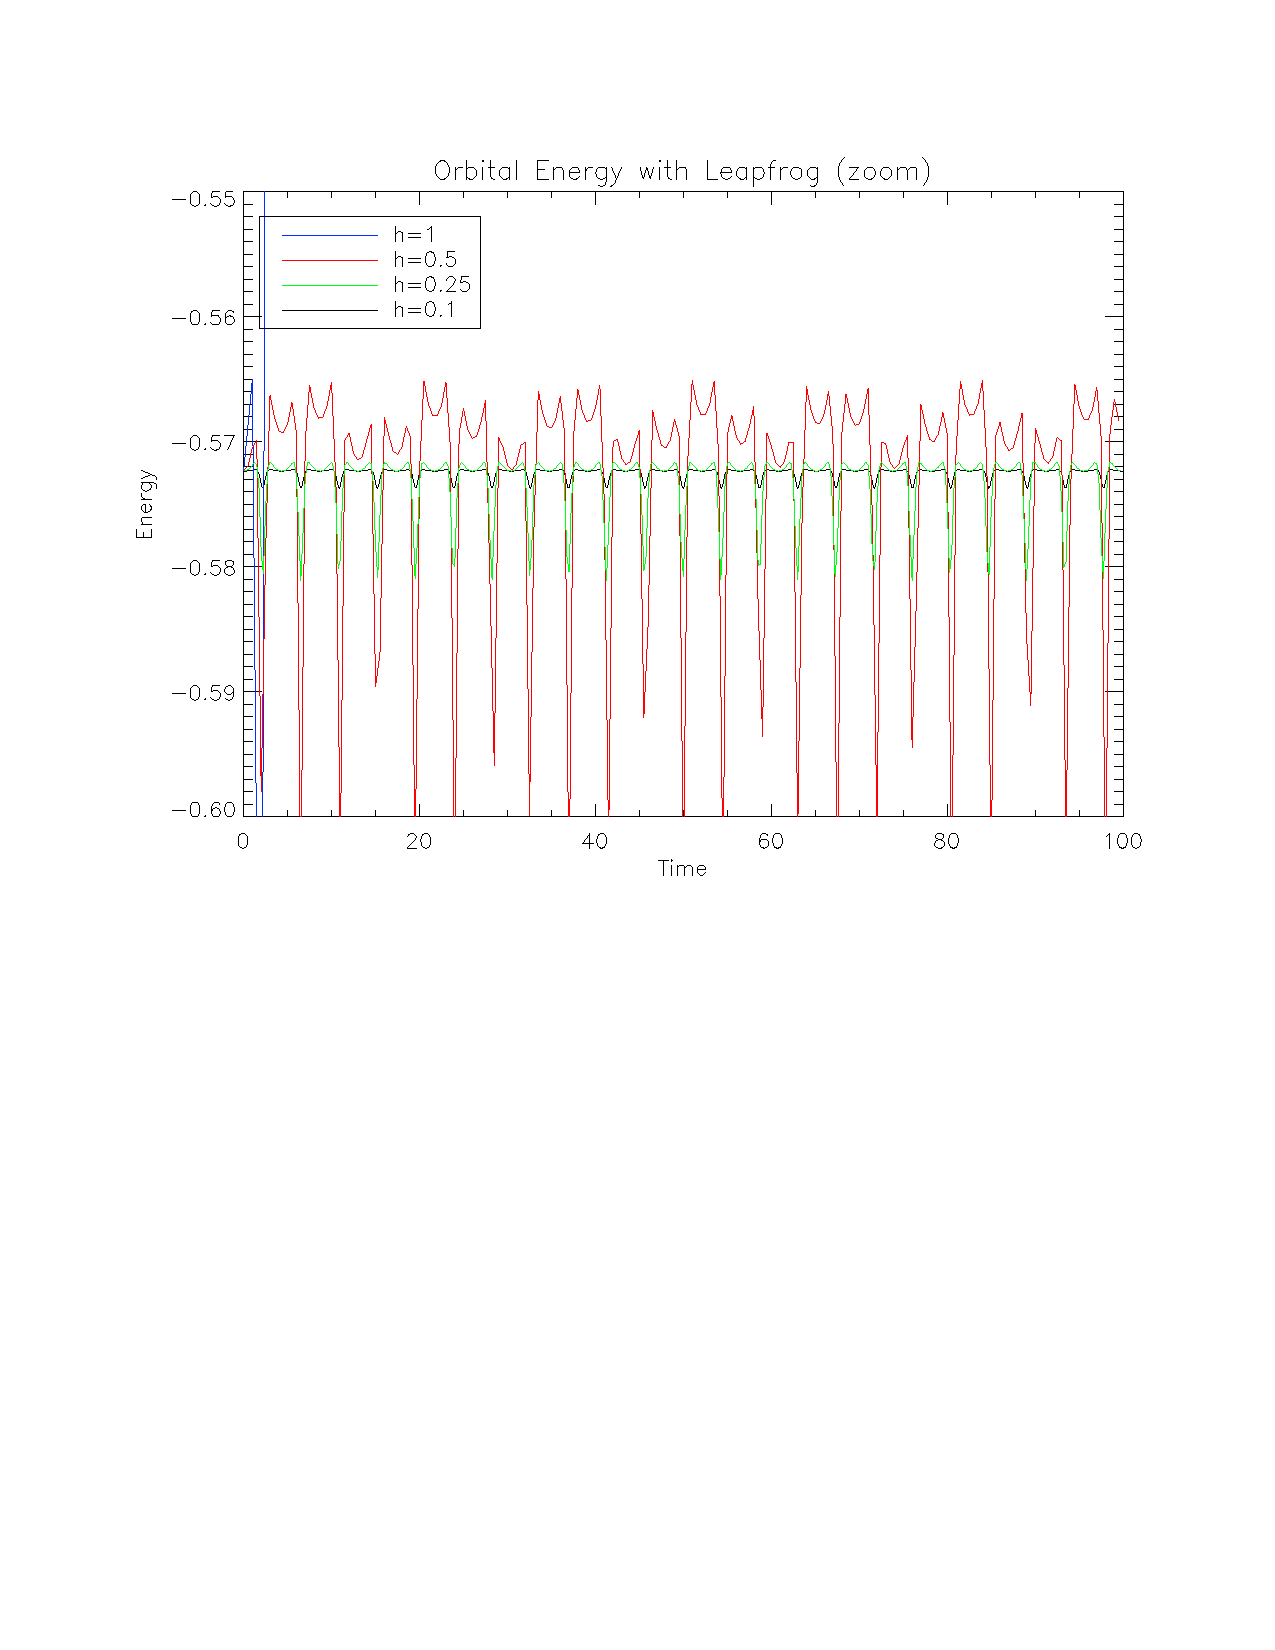
\includegraphics[scale = 0.7]{LFEnzoom.pdf}
\caption{}
\end{figure}
\begin{figure}
\centering
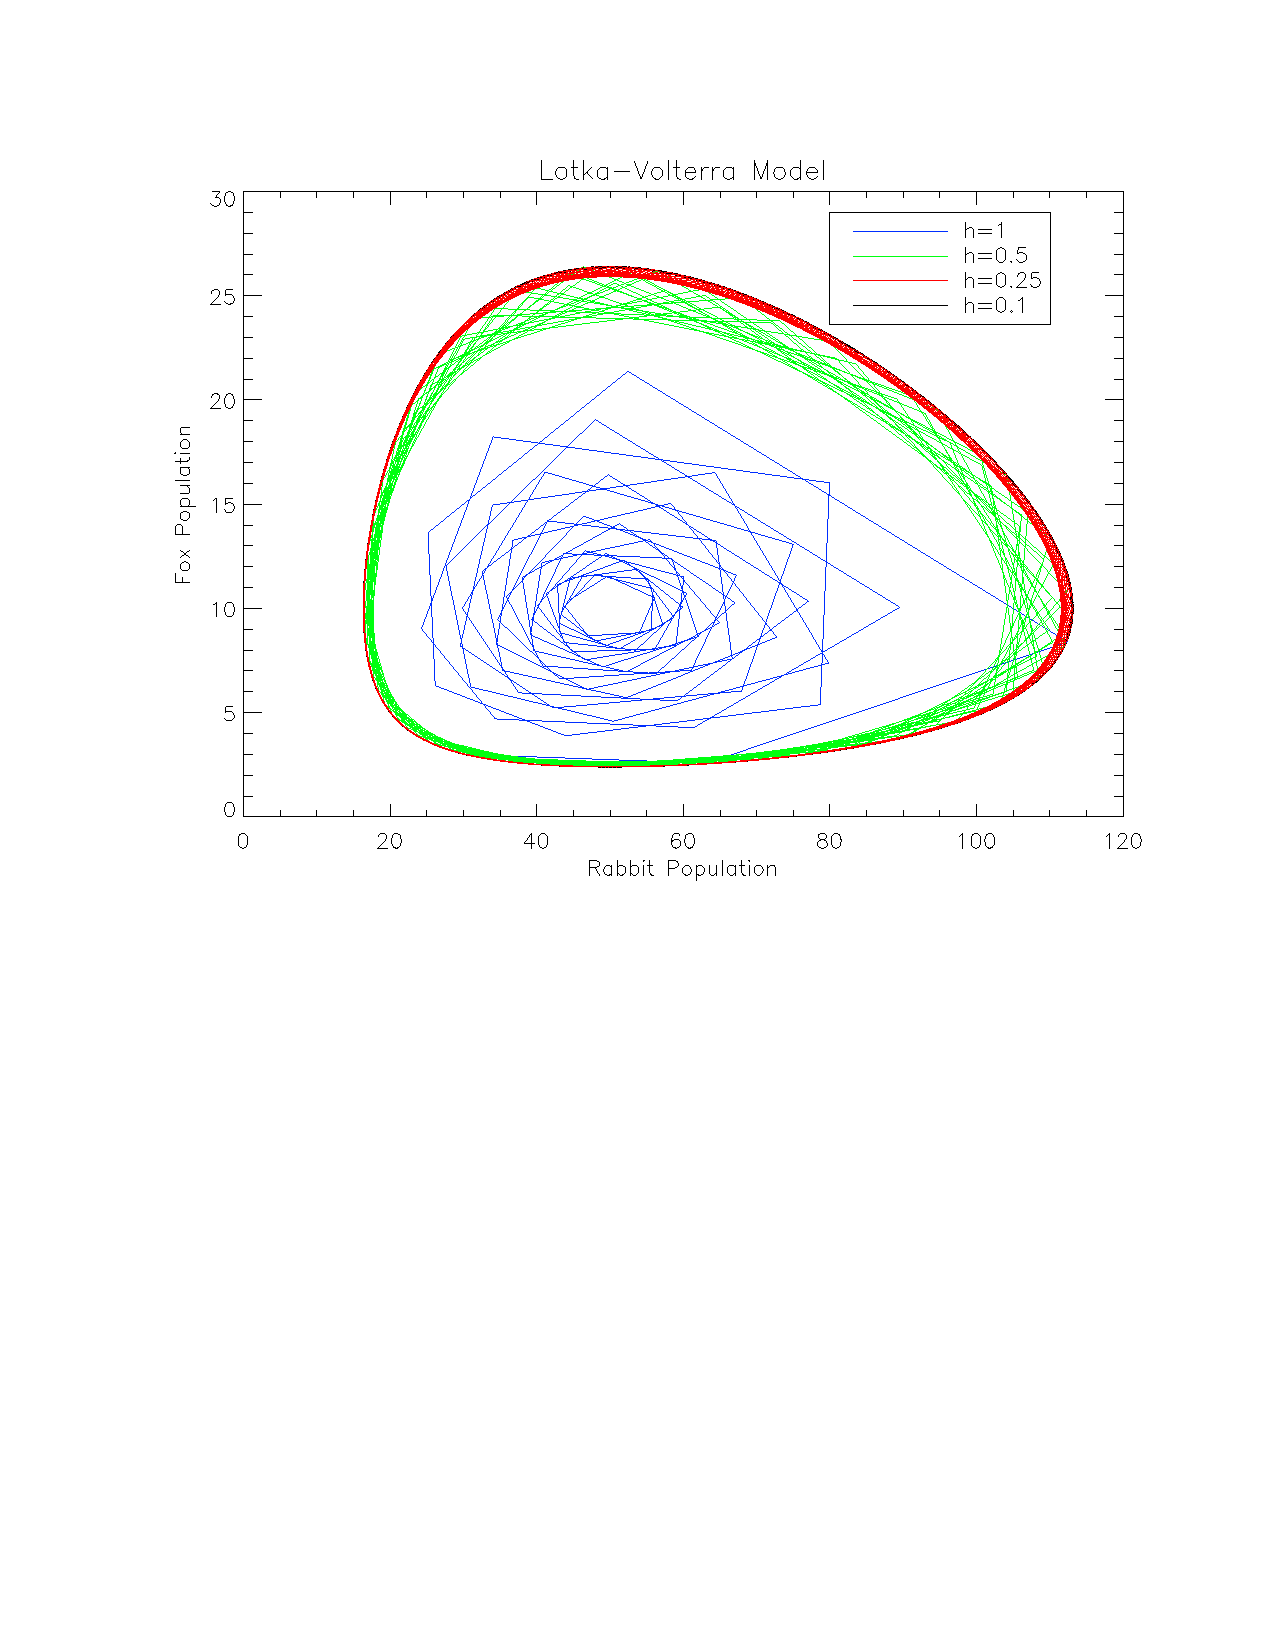
\includegraphics{Prey.pdf}
\caption{}
\end{figure}
\begin{figure}
\centering
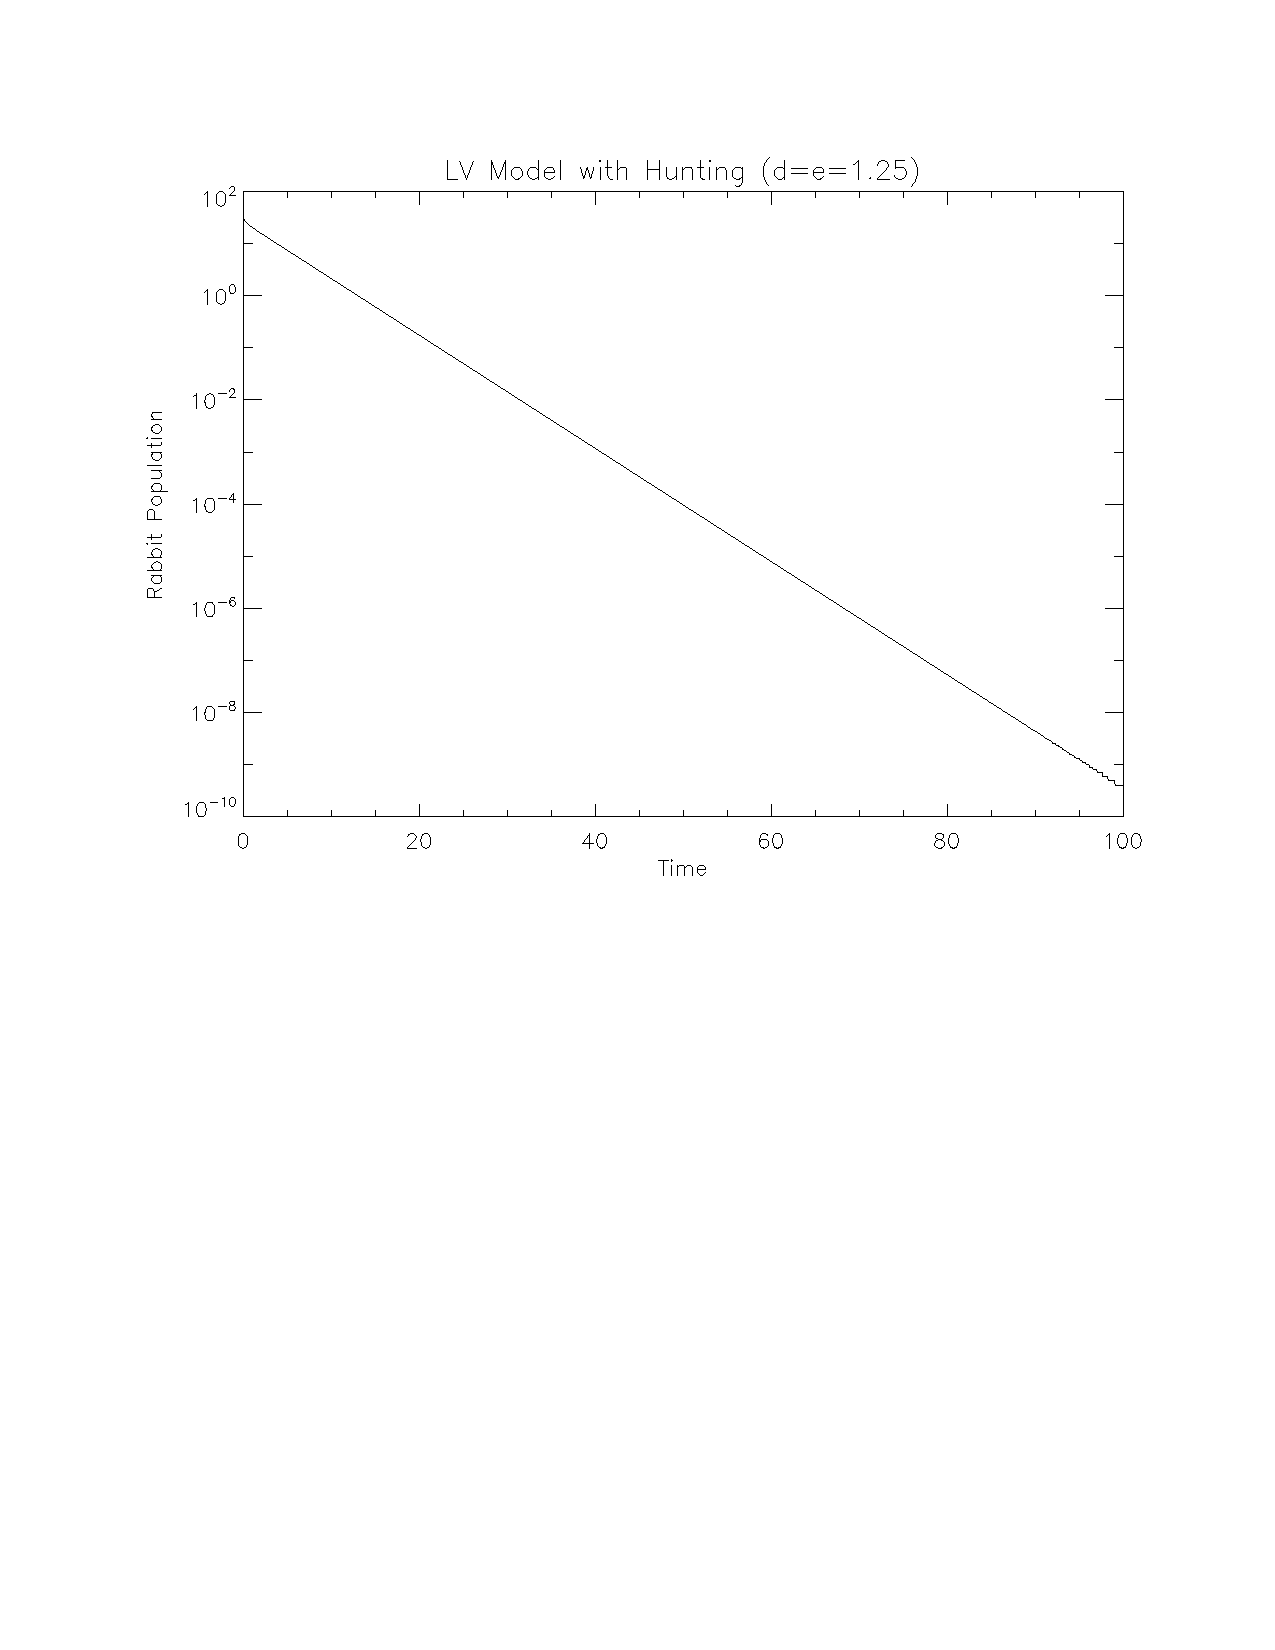
\includegraphics{Preyhunt.pdf}
\caption{}
\end{figure}



\end{document}

